%%%%%%%%%%%%%%%%%%%%%%%%%%%%%%%%%%%%%%%%%%%%%%%%%%%%%%%%%%%%%%%%%%%%%
%%                                                                 %%
%%           Simulador de inundaciones                             %%
%%           Proyecto fin de carrera                               %%
%%                                                                 %%
%%                            Alejandro Blanco Escudero            %%
%%                                  Manuel Gomar Acosta            %%
%%                                                                 %%
%%%%%%%%%%%%%%%%%%%%%%%%%%%%%%%%%%%%%%%%%%%%%%%%%%%%%%%%%%%%%%%%%%%%%

%     Copyright (C)  2010  Alejandro Blanco & Manuel Gomar
%     Permission is granted to copy, distribute and/or modify this document
%     under the terms of the GNU Free Documentation License, Version 1.3
%     or any later version published by the Free Software Foundation;
%     with no Invariant Sections, no Front-Cover Texts, and no Back-Cover Texts.
%     A copy of the license is included in the section entitled "GNU
%     Free Documentation License".

\documentclass[a4paper,12pt]{book}

%%  Include con la definición de estilos del usuario
%%%%%%%%%%%%%%%%%%%%%%%%%%%%%%%%%%%%%%%%%%%%%%%%%%%%%%%%%%%%%%%%%%%%%
\input definl

%%  Paquetería necesaria de fábrica
%%%%%%%%%%%%%%%%%%%%%%%%%%%%%%%%%%%%%%%%%%%%%%%%%%%%%%%%%%%%%%%%%%%%%
\usepackage[utf8x]{inputenc}
\usepackage{hyperref}
% \usepackage{palatino}
\usepackage[dvips]{graphicx} % para importar combinados latex
% \usepackage{color}           % para importar dibujos coloreados
% \usepackage{rotating}        % para usar \begin{sideways} que rota tabla 90
                             % grados
% \usepackage{epsfig}          % para rotar figuras de Xfig  poniendo
                             % \begin{sideways}
\usepackage{amsmath}         % para fórmulas matemáticas
% \usepackage{stmaryrd}        % para usar la \bigsqcap
% \usepackage{verbatim}        % para poner salidas de pantallas
\usepackage{listings}        % para imprimir codigo fuente
% \usepackage{shortvrb}

%%  Configuración de paquetes
%%%%%%%%%%%%%%%%%%%%%%%%%%%%%%%%%%%%%%%%%%%%%%%%%%%%%%%%%%%%%%%%%%%%%
\renewcommand\lstlistingname{Listado}                   %  default is Listing
\renewcommand\lstlistlistingname{\'Indice de listados}  %  default is Listings
% \renewcommand\thelstlisting{\thechapter .\arabic{lstlisting}} % captionstyle
\lstset{
  language=Java,
  basicstyle=\small,
  keywordstyle=\bfseries,
  showstringspaces=false,
  numbers=left,
  numberstyle=\tiny,
  stepnumber=1,
  numbersep=5pt,
  frame=single}

%%  Configuraciones varias
%%%%%%%%%%%%%%%%%%%%%%%%%%%%%%%%%%%%%%%%%%%%%%%%%%%%%%%%%%%%%%%%%%%%%
% \newcommand{\corregir}{\color{blue}}   % pintar en color azul
\setlength{\parskip}{2ex}              % después del párrafo, doble línea

% Para que no aparezcan las cabeceras de las páginas que están en blanco
%%%%%%%%%%%%%%%%%%%%%%%%%%%%%%%%%%%%%%%%%%%%%%%%%%%%%%%%%%%%%%%%%%%%%
\makeatletter
\def\cleardoublepage{\clearpage\if@twoside \ifodd\c@page\else
  \hbox{}
  \thispagestyle{empty}
  \newpage
  \if@twocolumn\hbox{}\newpage\fi\fi\fi}
\makeatother

%%  Cortes de palabras especiales
%%%%%%%%%%%%%%%%%%%%%%%%%%%%%%%%%%%%%%%%%%%%%%%%%%%%%%%%%%%%%%%%%%%%%
\hyphenation{
% de-sig-na
% for-mu-las
% de-se-chan-do-lo
}

\begin{document}

%%  Título e Índices
%%%%%%%%%%%%%%%%%%%%%%%%%%%%%%%%%%%%%%%%%%%%%%%%%%%%%%%%%%%%%%%%%%%%%%
\pagenumbering{roman}
\thispagestyle{empty}

{
\thispagestyle{empty}
\begin{center}

\includegraphics{figuras/titulo/logous-moderno.ps}
\end{center}
\vspace*{0cm}
\Large
\begin{center}
{\normalsize \sc
Departamento de Ciencias de la Computación \\ e Inteligencia Artificial \\}

\end{center}

\vspace{0.5cm}

\LARGE

\begin{center}
{\bf Simulador de Inundaciones. \\ Sistema Multiagente}
\end{center}

\Large

\vspace*{2cm}
\vfill

\hspace*{.5\textwidth}
\normalsize
\begin{tabular}{l}

Proyecto Fin de Carrera presentado\\
por Alejandro Blanco Escudero \\
y Manuel Gomar Acosta \\

\end{tabular} \par

\vspace*{-2.9cm}

Tutores

\vspace*{4cm}

D. Joaquín Borrego Díaz\newline
D. Gonzalo A. Aranda Corral\newline

Sevilla, 1 de Julio de 2010 % \today

\newpage
\thispagestyle{empty}
\mbox{ }
\newpage
\thispagestyle{empty}

\newpage
\thispagestyle{empty}

\mbox{ }

\vfill

\begin{flushright}
\begin{minipage}{9cm}
%    \em{``El hombre es inteligente porque tiene manos''}\\ \\
%Anaxágoras
%     \em{``Iré a cualquier parte, siempre que sea hacia delante.''}\\ \\
%David Livingston.
\em{''Nunca permití que la escuela interfiriera en mi educación.''}\\ \\
Mark Twain
\end{minipage}
\end{flushright}

\vfill

\newpage
\thispagestyle{empty}
\mbox{ }

}

\clearpage
\pagestyle{plain}
\tableofcontents
\clearpage
\listoffigures
\lstlistoflistings

%%  Contenido del trabajo
%%%%%%%%%%%%%%%%%%%%%%%%%%%%%%%%%%%%%%%%%%%%%%%%%%%%%%%%%%%%%%%%%%%%%%
\pagenumbering{arabic}
\pagestyle{fancy}
% Introducción
%     - Motivación
%     - Solución
%     - Estructura de la memoria

\chapter*{Introducción} \label{cap0}
\addcontentsline{toc}{chapter}{Introducción}

\pagenumbering{arabic}

\begin{flushright}
\begin{minipage}{7.85cm}
    {\em Si la única herramienta que se tiene es un martillo, se pensará que
    cada problema que surge es un clavo.} \\  Mark Twain
\end{minipage}
\end{flushright}

\vspace*{5mm}

\section*{Motivación}

Los desastres naturales provocan enormes pérdidas, tanto personales como
materiales. Se hace un gran esfuerzo en preparar medidas y se realizan grandes
inversiones en material, y aún así siguen produciéndose tragedias cada vez que
una inundación, un terremoto, etc, azota a algún país.

Por ello resulta de vital importancia ser capaces de simular estos escenarios,
para poder comprobar los efectos del desastre y tomar las medidas adecuadas. El
conocimiento previo al desastre es la clave, y la única forma de obtenerlo es
la simulación.

Pero por desgracia realizar una simulación realista mediante métodos
tradicionales resulta extremadamente complejo, además de caro
computacionalmente. Por ello nosotros proponemos un simulador basado en agentes.

\section*{Solución}

Los sistemas multiagente son una técnica de inteligencia artificial que nos
permite abordar este problema desde un nuevo punto de vista. Un agente es una
entidad {\em inteligente} y autónoma, pero relativamente simple, y por lo tanto
computacionalmente ligera. Es la conducta combinada de estos agentes la produce
un resultado en conjunto {\em inteligente}, un comportamiento emergente que no
tiene por qué estar planeado desde un principio.

Con esta herramienta es posible diseñar un simulador cuya carga computacional
no sea inabarcable y que produzca resultados satisfactorios.

\subsection*{Objetivos}

Se pretende con este proyecto desarrollar la base de un {\bf Simulador de
Desastres}, centrándose en el caso de una inundación. El simulador ha de cumplir
las siguientes condiciones:

\begin{itemize}
 \item Ha de simular utilizando datos reales del terreno simulado. No tendría
sentido realizar una simulación si no se puede aprovechar la información
obtenida con ella.
 \item Ha de ser escalable y distribuido. Es imprescindible que se pueda
simular sobre áreas tan grandes como se quiera, y que simplemente añadiendo más
máquinas a la infraestructura de simulación esto sea posible.
 \item Ha de ser fácilmente extensible a otros desastres naturales. La
arquitectura del simulador ha de estar diseñada para que esta tarea no requiera
grandes modificaciones del código existente.
 \item Ha de respetar los estándares utilizados en los sistemas multiagente. En
concreto los estándares de comunicación entre agentes establecidos por la FIPA
\footnote{Foundation for Intelligent Physical Agents:
\url{http://www.fipa.org/}}.
 \item Ha de poder generar estadísticas sobre el estado de las personas
simuladas, para poder realizar comparaciones entre simulaciones, o con datos
reales.
\end{itemize}

Como caso guía utilizaremos las inundaciones que siguieron al {\bf huracán
Katrina} en la ciudad estadounidense de {\bf Nueva Orleans}, en el año 2005.
Hemos escogido este caso concreto por la gran cantidad de documentación
disponible.

\subsection*{Resultados}

Para la visualización de resultados se ha optado por dos métodos. Un visor
bidimensional que muestra la simulación en ``tiempo real'', y un generador de
KML\footnote{Keyhole Markup Language:
\url{http://www.opengeospatial.org/standards/kml/}}. KML es un estándar para la
representación de información geográfica, y se puede abrir con múltiples
visores, uno de los más conocidos es {\em Google Earth}.

Generar ficheros KML nos permitirá mostrar los resultados de la simulación
sobre imágenes satélite del terreno simulado, con gráficos en 3D del terreno y
con los edificios modelados también en 3D. De esta manera la representación de
los resultados estará mucho más cercana a la realidad y será más accesible y
sencilla de interpretar.

\section*{Software Libre}

Citando a Richard M. Stallman: {\em ``Las obras de conocimiento deben ser
libres, no hay excusas para que no sea así''}. Y de hecho no las hay, nosotros
no concebimos este proyecto de ninguna forma que no sea Software Libre.

El Software Libre es una cuestión de libertad: las personas deberían ser libres
para usar el software de todas las maneras que sean socialmente útiles. El
software difiere de los objetos materiales (como las sillas, los bocadillos o la
gasolina) en el hecho de que puede copiarse y modificarse mucho más fácilmente.
Estas posibilidades hacen al software tan útil como es; y creemos que los
usuarios de software deberían ser capaces de aprovecharlas.

Por Software Libre entendemos aquel que cumple las siguientes cuatro libertades:

\begin{enumerate}
\setcounter{enumi}{-1}
\item La libertad de usar el programa, con cualquier propósito.
\item La libertad de estudiar cómo funciona el programa y modificarlo,
adaptándolo a tus necesidades.
\item La libertad de distribuir copias del programa, con lo cual puedes ayudar a
tu prójimo.
\item La libertad de mejorar el programa y hacer públicas esas mejoras a los
demás, de modo que toda la comunidad se beneficie.
\end{enumerate}

Y persiguiendo estos objetivos utilizaremos la licencia \hyperref[ap1]{GPL}
(Licencia Pública General de GNU) en su versión 3 o posterior para nuestro
proyecto.

\section*{Estructura de la memoria}

Esta memoria está dividida en los siguientes capítulos:

\begin{description}
 \item[Simulación basada en agentes:] Donde se describen las características de
los sistemas multiagentes.
 \item[Planteamiento del problema:] Donde se describen las dificultades que hay
que abordar a la hora de simular una inundación.
 \item[Solución propuesta:] Donde se detalla el diseño del simulador
desarrollado.
 \item[Tecnología elegida:] Donde se habla de JADE y otros aspectos
técnicos del simulador.
 \item[Metodología e implementación:] Donde se explica cómo ha sido desarrollado
el proyecto.
 \item[Resultados:] Donde se muestran los resultados obtenidos al simular con
este proyecto.
 \item[Conclusiones y trabajo futuro:] Donde se comentan las ideas obtenidas y
las que quedan por desarrollar.
 \item[Apéndices:] Donde se encuentra el contenido adicional de la memoria.
  \subitem Licencia del Simulador
  \subitem IV Concurso Universitario de Software Libre
\end{description} % Introducción
% Simulación basada en agentes

\chapter*{Simulación basada en Agentes} \label{cap1}
\addcontentsline{toc}{chapter}{Simulación basada en Agentes}

\pagenumbering{arabic}

\begin{flushright}
\begin{minipage}{7.85cm}
    {\em Creo que para final de siglo el uso de las palabras y la opinión
    general habrán cambiado tanto, que uno podrá hablar sobre máquinas pensantes
    sin que le contradigan.} \\ Alan M. Turing
\end{minipage}
\end{flushright}

\vspace*{5mm}

\section*{Agentes Inteligentes}

% http://en.wikipedia.org/wiki/Intelligent_agent#A_variety_of_definitions

Una posible definición muy resumida de agente inteligente sería la siguiente:
{\em Un agente inteligente es una entidad autónoma que observa y actúa sobre un
entorno, y dirige su actividad en pos de uno o más objetivos}. Por supuesto
esta definición no abarca muchos matices, pero nos da una idea general que nos
sirve como punto de partida. La variedad de agentes es muy amplia, así como
su complejidad, que puede ir desde un sencillo agente puramente reactivo a uno
complejo que imite a una persona, por ejemplo.

Existen muchas definiciones de agentes inteligentes, todas ellas diferentes,
pero con puntos en común. Los puntos que se pueden extraer como fundamentales
para considerar a un proceso como agente inteligente son:

\begin{description}
 \item[Autonomía]Deben ser capaces de funcionar sin la intervención del usuario.
 \item[Reactividad]Han de poder observar su entorno, y responder a los eventos
 o cambios que se produzcan.
 \item[Pro-actividad]Para conseguir sus objetivos han de tomar decisiones y
 realizar acciones según una estrategia.
 \item[Comunicación]Deben poder comunicarse entre sí, compartir información, e
 incluso, cooperar para la consecución de sus objetivos.
\end{description}

Aunque existen agentes puramente reactivos, es difícil aplicarles la etiqueta
de {\em inteligentes}. Un grado de pro-actividad es imprescindible, aunque se
hace necesario encontrar un equilibrio entre la reactividad y la búsqueda
activa de objetivos.

\subsection*{Tipos de Agentes}

% http://en.wikipedia.org/wiki/Intelligent_agent#Classes_of_intelligent_agents

\subsubsection*{Reactivos}

\subsubsection*{Reactivos basados en Modelo}

\subsubsection*{Basados en Objetivos}

\subsubsection*{Basados en Utilidad}

\subsubsection*{Con capacidad de Aprendizaje}

\section*{Sistemas Multiagente (SMA)}

% http://en.wikipedia.org/wiki/Multi-agent_system

\subsection*{Métodos de comunicación}
 % Simulación basada en agentes
% del problema: Simulación de inundaciones

\chapter*{Simulación de Inundaciones} \label{cap2}
\addcontentsline{toc}{chapter}{Simulación de Inundaciones}

\pagenumbering{arabic}

\begin{flushright}
\begin{minipage}{7.85cm}
    {\em Sólo podemos ver un poco del futuro, pero lo suficiente para darnos
    cuenta de que hay mucho por hacer.} \\  Alan Turing
\end{minipage}
\end{flushright}

\vspace*{5mm}

\section*{Planteamiento del Problema}
%simular el agua, simular las personas, obtener información real

Nuestra simulación se basa en tres grandes pilares. El agua, las personas y la
ciudad. 

Para poder simular una inundación\cite{simulator} primero necesitamos saber
como se comporta el
agua, cosas básicas como que tiende a moverse hacia las zonas bajas del terreno
hasta cosas no tan básicas como dinámica de fluidos.

Por otro lado queremos simular la reacción que tendrían las personas ante una
inundación, por ello necesitamos saber desde la velocidad a la que pueden
desplazarse, hasta sus posibles reacciones ante la llegada de una inundación.

Por ultimo queremos que nuestro sistema sea global, de tal forma que no este
restringido solo a una zona concreta del planeta, por ello hemos utilizado
sistemas de información global, como por ejemplo ''Open Streets Maps'', o en
el caso de estados unidos, un servidor de alturas. Aunque siempre estemos a
expensas de la disponibilidad de los datos, siempre que los haya y sean
accesibles, los podremos utilizar.

\section*{El movimiento del agua}

Para simular el movimiento del agua, hemos contemplado muchas posibles
soluciones a la simulación, puesto que simular fluidos y mecánica de fluido no
es algo para nada trivial, nosotros hemos optado por una simplificación para
poder abordar el tema del movimiento del agua. Puesto que nuestro sistema no
esta pensado para trabajar en tiempo real, sino a intervalos de tiempo, no
estamos obligados a utilizar un modelo muy estricto del agua, por lo que optamos
por varias simplificaciones.

\subsection*{Mecánica de fluidos}

Como ya hemos comentado anterior mente nuestra intención no es hacer un sistema
de agentes para simular grandes cantidades de fluidos moviéndose por un terreno
irregular, con obstáculos y con cálculos exactos de velocidades. Tampoco nos
preocupamos de si los elementos que arrastra la inundación modifican su
trayectoria o comportamiento, puesto que este problema, ya sería en si el tema
de una tesis completa.

En esta simulación abordamos dos de los problemas del movimiento del agua, la
dirección y la velocidad de propagación.

\subsubsection*{Dirección del Agua}

Cuando se produce una inundación, es importante saber en que dirección se
propagará la masa de agua, puesto que necesitamos saber cuales serán los
terrenos afectos por la inundación.

La dirección del agua dependen de muchos factores, el mas determinante de ellos
es, debido a la energía potencial, la altura, el agua siempre va a tender a ir
desde donde se encuentra al punto mas bajo accesible.

Otro factor que influye en la dirección del agua, aunque en menor medida es la
fuerza inicial del agua y su velocidad, puesto que pueden desviar un poco la
corriente principal e incluso salvar obstáculos o subir hasta una determinada
altura en un terreno e inundar terrenos que sin tener en cuenta estos factores
nunca hubieran sido inundados.

Para resolver este problema nosotros solo disponemos de la altura del terreno
como único dato.

\subsubsection*{Velocidad de propagación del Agua}

La velocidad de propagación de un fluido en un entorno irregular es un problema
muy complejo, nos hemos visto 
obligados a simplificar muchísimo el sistema,
puesto que tener en cuenta
variables tales como la fuerza inicial del agua, dirección, la presión, la
ganancia o perdida de fuerza al bajar por un terreno o subir, el posible
desgaste del terreno o incluso su resistencia a paso del agua, al tener mas o
menos obstáculos que pudieran oponerse y frenar el agua. 

El problema no es que no seamos capaces de simular este sistema con nuestros
agentes, o que sea inabordable por su complejidad, sino que además no tenemos 
datos para poder recrear el escenario
esta simulación. Datos sobre la composición del terreno, los obstáculos,
resistencias de materiales, dureza, permeabilidad al agua ... no se encuentran
tan fácilmente.

\subsubsection*{Otros problemas con el agua}

Entre otros muchos posibles problemas que podríamos haber abordado por su
sencillez y por la versatilidad de nuestro sistema ya que el coste de
implementación habría sido muy bajo son, entre otros el problema de la absorción
de agua por parte del terreno, que podría no ser despreciable y por supuesto el
tema de las filtraciones de agua, puesto que el agua también podría moverse por
debajo de la tierra y llegar a zonas mas bajas sin tener contacto directo. Pero
una vez mas por falta de datos, se han tenido que quedar en el tintero.


\section*{Inundaciones en un entorno urbano}

Simular una inundación en un entorno urbano tiene sus propios problemas, tales
como la el papel de los ríos, las calles, la forma de los edificios, la red de
alcantarillado, etc... \cite{simulator, katrina}
\subsection*{Los ríos}
En una ciudad, un río será por lo general, un sector conflictivo cuando se
produzca una inundación, puesto que aparte de que probablemente sea el causante
de la inundación  también es una zona en la que pueden producirse.

Los cálculos necesarios para calcular el caudal introducido y caudal evacuado
\cite{desvordamiento} son complejos de por si, pero podrían ser resueltos por
nuestro sistema multi-agente, sin embargo el problema de la obtención de datos,
es mucho mas complicado, puesto que en muy pocas circunstancias se tiene
constancia de los datos necesarios.

\subsection*{La forma de los edificios}
La forma de los edificios también va a influir en el desarrollo de la
inundación, no solo en que cuando entre el agua dentro del edificio modificará
su velocidad y trayectoria, sino con las paredes o fachadas, que pueden
canalizar el agua e incluso formar piscinas en su interior o inundar sótanos.

Sin conocer la forma del edificio no podemos hacer una simulación del todo fiel
a realidad puesto que algunos terrenos serán afectados de forma diferente si
hay un edificio delante de ellos que frena el avance del agua, o si por el
contrario, un edificio hace de tapón y provoca un crecimiento anómalo del nivel
del agua.

\subsection*{Las calles y carreteras}
Las calles y carreteras tienen una peculiaridad, puesto que al ser
prácticamente planas y de inclinación suave las hacen idóneas para que el agua
pueda moverse sin mucha dificultad por la ciudad. Ya que a un nivel pequeño del
agua sirven como canales que conducen en agua hacia un lugar mas bajo pero a
mucha mas velocidad que si lo hicieran a través de los edificios o por cualquier
otra superficie no plana.

\subsection*{El alcantarillado}
Todas las ciudades tienen una red de alcantarillado, que no es mas que un
conjunto de canales que desplazan el agua desde la ciudad hasta un punto de la
ciudad. Por las redes del alcantarillado va a circular gran cantidad de agua
durante una inundación y no se verá afectada por la elevación del terreno ya
que al ser subterránea y estar canalizada va a llevar una gran cantidad de agua
a otro punto.

Este es un problema que se puede asemejar al de las filtraciones, pero con un
factor mucho mas alto.

Una vez mas habría que disponer de un mapa del alcantarillado y de sus zonas de
desagüe, aunque, se puede asumir que prácticamente debajo de cada carretera
habrá una alcantarilla, aún así se estarían ignorando muchos otros puntos de
entrada o salida de agua.

\subsection*{Prioridades de las personas}

Se han realizado estudios \cite{prioridades} sobre poblaciones acerca de que es
lo que harían en caso de crisis, tales como su disponibilidad a salvar a sus
familiares en apuros, o al vecino, o simplemente a alguien que lo necesite.
Nuestro problema podría ser simular comportamientos de ayuda entre agentes
tales como indicarles el camino a seguir o incluso acompañarles a un lugar
seguro.

\subsection*{Supervivencia en un entorno inundado}

También es importante ante una catástrofe, recoger información sobre los
supervivientes \cite{survey}.

Información como los peores momentos de la inundación, las zonas mas afectas,
las mayores concentraciones de personas y ese tipo de datos pueden darnos una
idea de como se podrían prevenir ciertas situaciones de riesgo.

También nos puede ser útil para prever un informe de daños y necesidades de la
población tras el desastre.

\subsection*{Evacuación de personas}
%como se evacuan las personas de una ciudad
La correcta evacuación de una ciudad ante un desastre es algo muy importante de
lo que pueden depender la vida de muchas personas, la rapidez y eficacia de la
evacuación puede determinar la magnitud de la catástrofe en vidas humanas. Por
ello, poder simular como se realizaría una simulación podría darnos datos de
rutas frecuentes de evacuación \cite{evac08} o en situaciones de pánico
\cite{panicevac} y concentrar las esfuerzos de las autoridades para mantener
estas vías abiertas, o en su defecto, detectar vías alternativas y posibles
problemas.

Otro problema a plantearse serían la evacuación de los edificios en si
\cite{kyoto}, puesto que en una gran ciudad, tan importante es la evacuación de
las calles, como de los grandes edificios donde se encuentran la mayoría de la
gente.
 

\section*{Obtener información real sobre los terrenos}
%obtención de información global

Lo verdaderamente interesante de nuestro proyecto es poder probarlo sobre
lugares reales, para ello es necesario obtener la información, pero además,
decidimos hacerlo de tal forma de que el lugar no fuera el problema, siempre que
tengamos datos de ese lugar, podremos integrarlos en nuestro simulador y simular
el problema allí donde se encuentre. Para ello necesitábamos usar un sistema de
geolocalización y servidores de información globales.

Sin embargo para los servidores de información lo teníamos mas difícil al no
existir servicios a nivel global, al menos, disponibles al publico.

\subsection*{Elevación del terrenos}

No existe, o al menos no conocemos un servidor global de alturas.

Por lo que de momento, solo disponemos de un servicio de alturas para el caso de
nuestro estudio, ''Nueva Orleans''.

Si embargo, como ya hemos comentado antes, nuestra pretensión es que la
simulación se pueda realizar en cualquier parte del planeta, por lo que la
nuestro sistema esta preparado para poder añadirle fácilmente otros servidores a
fin de poder simular en cualquier otro lugar. 

\subsection*{Posibles rutas de evacuación}

Con nuestro simulador no solo pretendemos simular la inundación en sí, sino la
posible reacción de las personas ante la inundación, para ello, como ya hemos
visto antes, necesitamos saber que es lo que las personas harían ante una
crisis y además, conocer la ciudad en sí en la que se desarrolla, sobre todo sus
calles, puesto que es probablemente, la ruta mas probable de la ciudad.
En una evacuación ante una inundación es muy importante conocer el plano de la
ciudad, para poder registrar las posibles rutas de de evacuación.

Para obtener los planos de las ciudades optamos por ''Open Streets Map'' ya que
al ser un estándar abierto y con información de ciudades a nivel global pues
tenía todo lo que le pudiéramos necesitar. 

También contiene mucha información adicional, tales como parques, hospitales,
aeropuertos, y lugares de interés que podrían ser identificados como puntos de
salvamento, o al menos objetivos para los evacuados.

Gracias a este servicio obtenemos también la posición y forma de los ríos,
mares, puentes ... muy importantes para las inundaciones. 

Nuestro problema ahora se centraría en adaptar esos datos de forma que pudieran
ser codificados e interpretados por nuestro simulador, no solo trazando calles
y carreteras por nuestro simulador, sino reconociendo posibles puntos de
salvamento o objetivos de los evacuados.

\section*{Geolocalización}

Nosotros queremos simular en terrenos reales, y los terrenos vienen
localizados por coordenadas geográficas (WGS84).

Gracias a las coordenadas podemos obtener información geolocalizada de
cualquier parte del mundo e identificarla con esa zona.

Por lo que nos encontramos con el problema de la discretización de los
datos y la inevitable perdida de información.

\subsection*{Discretización de los Datos}
Muchas veces, debido a que nosotros trabajamos sobre un mapa hexagonal, al
hacer el cambio desde coordenadas geográficas, dependiendo del nivel de
precisión de nuestra rejilla, inevitablemente vamos a sufrir una perdida de
información.

Otras veces los datos recibidos de las localizaciones no son del todo exactos o
precisos, como por ejemplo las localizaciones de los edificios, que vienen
representadas por el centro del edificio, y no por su perímetro, por lo que a
veces nos veremos obligados a aproximar puntos o a cambiarlos un poco de sitio.

Por ello pueden aparecer calles de un tamaño mayor al real o incluso un poco
desplazadas, pero suponemos que eso no tendrá consecuencias mayores.

\section*{Visualización de los Resultados}

Nuestra intención no es solo simular una inundación, si no que se pueda ver,
paso a paso, la evolución de esta misma. 

Esto conlleva los siguiente:
\begin {itemize}
\item Necesidad de conocer en que paso de la simulación nos encontramos.
\item Llevar un historial de la inundación.
\item Realizar la inundación ordenadamente.
\end {itemize}

\subsection*{Visor Simple}
Para las primeras fases del desarrollo y para poder ver de una forma simple y
sin ayuda de programas externos, necesitamos un visor nativo del sistema, con
el que poder seguir el progreso y comportamiento del agua y de los demás
agentes implicados en la simulación.
\subsection*{Kml}

Una vez terminada la simulación, queremos poder tener un historial de todo lo
que haya ocurrido y la facilidad de poder navegar dentro de la simulación para
poder recrear el estado de la simulación en un momento preciso.

Para ello dispondremos de un sistema que guarde la información de cada
instantánea de la simulación dentro de un fichero Kml.

Hemos elegido Kml debido a que es un estándar y a la versatilidad y potencia
gráfica que nos proporciona.

Utilizar Kml también nos obligará a tratar con problemas de geometría
computacional, y de topología. 

\subsection*{Estadísticas}
Una buena forma de comparar entre los distintos comportamientos implementados
para el agua o las personas o cualquier otro agente, son las estadísticas, así
que tendremos que crear un sistema que sea capaz de recoger estadísticas de tal
forma que nos puedan dar información importante sobre la simulación y así poder
discernir entre que métodos o estrategias son mejores con respecto a que
objetivos. % Planteamiento del problema
% Solución propuesta (diseño) % Solución propuesta
\chapter*{Tecnología Elegida} \label{cap4}
\addcontentsline{toc}{chapter}{Tecnología Elegida}

\begin{flushright}
\begin{minipage}{7.85cm}
    {\em Cualquier tecnología lo suficientemente avanzada es indistinguible de
    la magia.} \\ Arthur C. Clarke
\end{minipage}
\end{flushright}

\vspace*{5mm}

\section*{Licencias}

Para este proyecto vamos a usar la licencia GPL (Licencia Pública General de
GNU) en su versión 3 o posterior, escrita y mantenida por la FSF\footnote{Free
Software Foundation: \url{http://www.fsf.org/}}. El texto legal se puede
encontrar en el \hyperref[ap1]{Apéndice primero}.

Al colocar el simulador bajo esta licencia nos tenemos que asegurar que todas
las librerías que utilicemos estén bajo licencias compatibles con la nuestra. A
continuación sigue un gráfico con la relación de compatibilidad de otras
licencias libres con la GPL v3.

\begin{figure}[H]
 \centering
 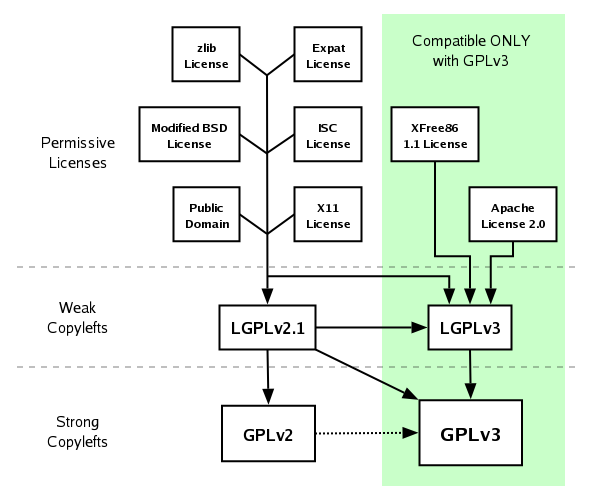
\includegraphics[width=120mm]{figuras/cap4/gplv3_comp.png}
 \caption{Compatibilidad de otras licencias libres con la GPL v3}
\end{figure}

\section*{JADE}

La plataforma JADE (Java Agent DEvelopment Framework) es la escogida para el
desarrollo del simulador. El objetivo principal de esta plataforma es la
simplificación del desarrollo de sistemas multiagentes, siguiendo a su vez los
estándares de comunicación entre sistemas de la FIPA\footnote{Foundation for
Intelligent Physical Agents: \url{http://www.fipa.org/}}. FIPA es una
organización internacional sin ánimo de lucro dedicada a establecer un marco
común y genérico, para el desarrollo de agentes y sistemas multiagente.

\begin{figure}[H]
 \centering
 
\includegraphics[width=30mm]{figuras/cap4/jade.png}
 \caption{Logo de JADE}
\end{figure}

JADE está desarrollado y mantenido por Telecom
Italia\footnote{\url{http://jade.tilab.com/}}, y es una plataforma para el
desarrollo de sistemas multiagentes.

Al utilizar JADE el desarrollador sólo tiene que concentrarse en los agentes
que escriba, el resto de aspectos del sistema están ya resueltos, tales como el
intercambio de mensajes, la búsqueda de agentes, el ciclo de vida de estos,
etc. Además está escrita en Java, lo que aumenta la portabilidad a múltiples
entornos de ejecución frente otros lenguajes de programación.

Dado que nuestro proyecto hace uso de la licencia \hyperref[ap1]{GPL v3}, es
vital que el software que utilicemos sea también libre y esté bajo una licencia
compatible. En concreto JADE usa la licencia LGPL\footnote{Licencia Pública
General Reducida de GNU:
\url{http://www.gnu.org/licenses/old-licenses/lgpl-2.0.html}} v2.

Además de ser Software Libre, JADE tiene también la virtud de cumplir con la
especificación completa de la FIPA. Cumplir con dichos estándares es muy
importante para que sea posible la interacción entre sistemas multiagentes, y
que el proyecto no sea un entorno cerrado sin capacidad de comunicación.

Por todos estos motivos hemos escogido esta tecnología de agentes. El hecho de
utilizar JADE nos condiciona a utilizar Java como lenguaje y plataforma de
desarrollo para el proyecto. El resto de librerías y paquetes que utilizamos, y
que describimos en los siguientes apartados, están pues escritos en este
lenguaje.

\subsection*{Arquitectura FIPA}

Como ya hemos mencionado, JADE implementa por completo la arquitectura de
sistemas multiagentes de la FIPA. Esta arquitectura ha sido desarrollada por
FIPA con el objetivo de permitir la construcción de sistemas multigente que se
integren entre sí en un entorno de computación particular. Adicionalmente
podrían interoperar con sistemas construidos con diferente tecnología pero que
también sigan estas especificaciones, todo ello con el mínimo esfuerzo.

\begin{figure}[H]
 \centering
 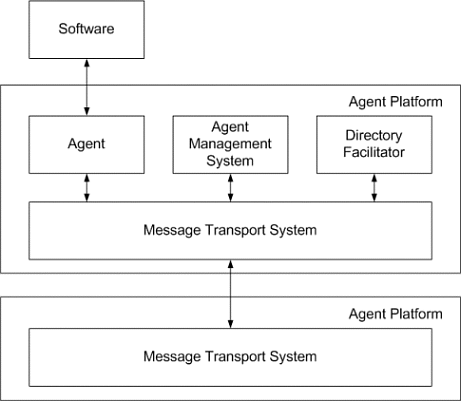
\includegraphics[width=100mm]{figuras/cap4/fipa.png}
 \caption{Arquitectura de la plataforma FIPA}
\end{figure}

FIPA establece el modelo lógico referente a la creación, destrucción, registro,
localización y comunicación de agentes. Según las especificaciones, los agentes
han de estar siempre conectados a una plataforma para poder funcionar, esto es
así debido a que su ciclo de vida es gestionado por la plataforma.

\begin{figure}[H]
 \centering
 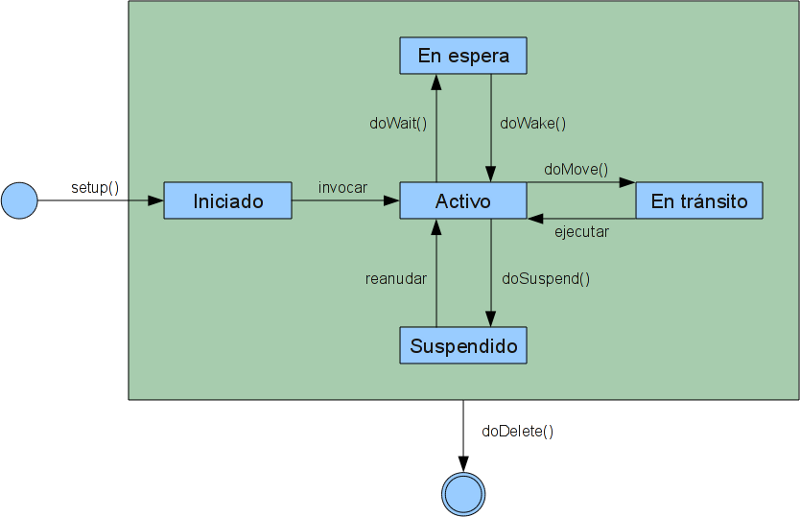
\includegraphics[width=130mm]{figuras/cap4/fipa_agent.png}
 \caption{Ciclo de vida de un agente FIPA}
\end{figure}

Cuando un agente se conecta a una plataforma, se produce un registro de éste
en la misma, habitualmente de manera implícita; aunque en caso de agentes
móviles que se trasladen de una plataforma a otra, por ejemplo, el registro debe
ser explícito. Este registro es necesario para que el resto de agentes puedan
localizarlo y comunicarse con él.

El estándar FIPA también define los servicios que debe proporcionar toda
plataforma de agentes, a saber:

\begin{itemize}
 \item Un sistema encargado del transporte de mensajes (Internal Platform
 Message Transport y Message Transport System).
 \item Un sistema de gestión de agentes (Agent Management System).
 \item Un servicio de directorio (Directory Facilitator).
 \item Un canal de comunicaciones para los agentes (Agent Communication Chanel).
\end{itemize}

Cada uno de estos servicios, excepto el de transporte de mensajes, es
suministrado por agentes especializados. Esto supone que la comunicación con
ellos será mediante mensajes ACL (Agent Communication Language) y utilizando una
ontología definida para dicho servicio.

\subsubsection*{Agent Management System}

% TODO

\subsubsection*{Directory Facilitator}

\subsubsection*{Agent Communication Channel}

\subsubsection*{Agent Communication Language}

\section*{Java}

Java es un lenguaje de programación orientado a objetos desarrollado por Sun
Microsystems, recientemente adquirida por Oracle, a principios de los años 90.
El leitmotiv de los desarrolladores de Java era {\em write once, run anywhere},
que hace referencia a la portabilidad de un programa Java, capaz de ejecutarse
allá donde hubiera una máquina virtual, una de las características más notorias
de la plataforma.

La elección de utilizar Java viene condicionada a la elección de utilizar JADE,
que está escrito en este lenguaje.

De Java existe una implementación totalmente libre de nombre
OpenJDK\footnote{\url{http://openjdk.java.net/}}. OpenJDK soporta el 99\% de la
plataforma, y el simulador podrá ejecutarse sobre esta implementación.

\section*{JAK}

JAK (Java API for KML) son un conjunto de librerías para el manejo de ficheros
KML desde Java. JAK ha sido desarrollado por Micromata
GmbH\footnote{\url{http://labs.micromata.de/display/jak/Home}}.

\begin{figure}[H]
 \centering
 
\includegraphics[width=30mm]{figuras/cap4/jak.png}
 \caption{Logo de JAK}
\end{figure}

Al igual que en el caso de {\bf JADE} es necesario que JAK sea compatible con
la licencia de nuestro proyecto, la \hyperref[ap1]{GPL v3}.
Los desarrolladores de JAK optaron por liberar las librerías bajo una licencia
BSD\footnote{Berkeley Software Distribution:
\url{http://www.opensource.org/licenses/bsd-license.php}} de 3 clausulas, o como
también se la conoce, licencia BSD modificada o nueva licencia BSD. La licencia
de JAK se puede consultar en su sitio web.

Gracias a JAK podremos generar los ficheros KML con el resultado de la
simulación.

\section*{Jcoord}

Para el manejo de coordenadas geográficas utilizaremos
Jcoord\footnote{\url{http://www.jstott.me.uk/jcoord/}}, un paquete de clases que
nos permitirán convertir entre formatos de coordenadas, calcular distancias,
etc. Jcoord ha sido desarrollado por Jonathan Mark Stott, y tal como se puede
consultar en su sitio web está licenciado bajo GPL v2, compatible con nuestra
\hyperref[ap1]{GPL v3}.

Además del habitual sistema de coordenadas latitud/longitud
WGS84\footnote{Sistema Geodésico Mundial 1984} soporta UTM\footnote{Sistema de
Coordenadas Universal Transversal de Mercator}.

A diferencia de {\bf JADE} o {\bf JAK}, integraremos directamente el código en
el simulador, por lo que no será una dependencia. De esta manera podremos
modificar y adaptar el paquete a nuestras necesidades.

\section*{Otras librerías}

\subsection*{Java CSV}

Java CSV\footnote{\url{http://sourceforge.net/projects/javacsv/}} es una
sencilla librería que facilita la escritura y lectura de ficheros de valores
separados por coma. Lo utilizaremos para escribir en ficheros los datos del
módulo de estadísticas.

La licencia de esta librería es la LGPL v2.1 o posterior, y estará integrada en
el código del proyecto por lo que no será una dependencia.

\subsection*{OpenWFE}

Del proyecto OpenWFE\footnote{Open WorkFlow Engine:
\url{http://sourceforge.net/projects/openwfe/}} en realidad sólo utilizaremos
una clase. Una implementación de Wget en Java (una herramienta para descargar
ficheros de la web). La licencia de OpenWFE es una BSD de 3 clausulas.

Dicha clase estará integrada en el código del simulador por lo que OpenWFE no
será una dependencia.

\section*{Servicios}

Además de las librerías comentadas hasta ahora haremos uso de algunos
servicios, como son Open Street Maps y el servicio web de elevaciones de la
USGS descritos en \hyperref[cap3]{el capítulo 3}.

\subsection*{Open Street Maps}

Open Street Maps (OSM)\cite{Pinto09} permite que se le realicen peticiones GET
por HTML, y
devuelve directamente un fichero con la información solicitada en
XML\footnote{Lenguaje de Marcado Extensible: \url{http://www.w3.org/XML/}}. La
implementación de la petición será por lo tanto sencilla, aunque el tratamiento
de los datos recibidos requerirá de un procesado mucho más complejo.

\begin{figure}[H]
 \centering
 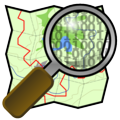
\includegraphics[width=20mm]{figuras/cap4/osm.png}
 \caption{Logo de Open Street Maps}
\end{figure}

\subsection*{Servicio de elevaciones de la USGS}

La U.S. Geological Survey (USGS) proporciona un método para obtener la elevación
del terreno si éste pertenece a los Estados Unidos. Este servicio consiste en un
servicio web al que se accede a través de SOAP\footnote{Simple Object Access
Protocol: \url{http://www.w3.org/TR/soap/}}. Para consumir dicho servicio hace
falta implementar un cliente, tarea que gracias a Java resulta bastante
sencilla.

Utilizaremos la herramienta {\bf wsimport} que trae Java para autogenerar el
código del cliente del servicio web, código que irá incluido en el proyecto.

\begin{figure}[H]
 \centering
 
\includegraphics[width=35mm]{figuras/cap4/usgs.png}
 \caption{Logo de la USGS}
\end{figure}

%%% Local Variables:
%%% mode: latex
%%% TeX-master: "../dissim"
%%% End: % Tecnología elegida
% Metodología e implementación

\chapter*{Implementación} \label{cap5}
\addcontentsline{toc}{chapter}{Implementación}

\begin{flushright}
\begin{minipage}{7.85cm}
    {\em Si necesitas más de tres niveles de indentación estás jodido, y
    deberías arreglar tu programa.} \\  Linus Torvalds
\end{minipage}
\end{flushright}

\vspace*{5mm}

\section*{Metodología}

Al ser este un proyecto de tamaño considerable, y al realizarse en grupo, es
necesario establecer una metodología para evitar el trabajo inútil o redundante.

Para organizar nuestro trabajo, y poder mantener siempre cierto control sobre la
evolución de la aplicación, nos hemos servido tanto de herramientas como de
algunas buenas prácticas.

Habiendo desarrollado nuestro proyecto en el marco del IV CUSL\footnote{Concurso
Universitario de Software Libre: \url{http://www.concursosoftwarelibre.org}}
hemos seguido una política de divulgación de la información y unos plazos de
entrega. Desde la organización del concurso pusieron a nuestra disposición una
forja, en concreto la forja
IRIS-Libre\footnote{\url{https://forja.rediris.es/projects/cusl4-catastrof/}},
gracias a la que pudimos agilizar y centralizar las labores de administración y
planificación del proyecto.

Además adoptamos una política de entrevistas frecuentes con los tutores para
así motivarnos y que nos aconsejaran sobre el mejor paso a seguir, o en dónde
deberíamos profundizar más, o cuándo seguir otras vías de investigación.

De esta manera teníamos objetivos a corto plazo, herramientas para la
planificación gracias al IV CUSL, y guía por parte de los tutores.

\subsection*{Metodologías Ágiles}

Una buena planificación no implica el éxito, pero por lo menos te asegura unos
resultados mínimos.

No hemos aplicado ninguna metodología en concreto, si no un conjunto de técnicas
y buenos métodos. Creemos en una metodología de desarrollo ágil.

\subsubsection*{Reuniones de Desarrollo}

Lo principal es la comunicación entre los desarrolladores, para ello decidimos
reunirnos y comentar las avances o principales problemas al menos dos veces a
la semana.

Las reuniones no tenían por qué ser en persona, ni muy formales, podían
realizarse a través de mensajería instantánea, ayudados con herramientas de
pizarras virtuales. De esta forma siempre se tiene una idea muy cercana del
desarrollo del proyecto sin perder mucho tiempo.

Además mantiene un fuerte lazo entre los desarrolladores y les permite ayudarse
unos a otros, evitando así estancamientos o frustraciones con problemas
difíciles.

\subsubsection*{Reuniones con los Tutores}

Nos reuníamos con nuestros tutores al menos dos veces al mes, dependiendo del
ritmo de trabajo y progresos. Estas reuniones eran de carácter informativo y
orientativo.

Las reuniones permiten un crecimiento guiado y controlado del producto final, y
un nivel de acabado mayor al centrarnos solo en las partes realmente importantes
de la investigación y el desarrollo para los objetivos del proyecto.

\subsubsection*{Sistema Incremental}

Lo principal era desarrollar una plataforma muy básica y sencilla donde se
pudieran llevar a cabo pruebas, y una vez completada, ir aumentando las
prestaciones en forma de módulos o complementos que fueran implementando las
funcionalidades deseadas.

Seguimos pues un modelo iterativo de desarrollo del software, que es el ciclo
de vida del software que probablemente mejor se adapte a metodologías ágiles.

% TODO esquema del ciclo de vida iterativo

\subsubsection*{Reparto de Tareas Dinámico}

El reparto de tareas equitativo y ágil es vital para mantener una buena
relación entre los desarrolladores, y para el adecuado progreso del proyecto.

Por ello es importante identificar las tareas a realizar e ir asignándolas a
los desarrolladores, de forma que ellos mismos puedan decidir cómo organizarse,
pero siempre teniendo en cuenta unos plazos finales.

El reparto no siempre es estático, puesto que las tareas se pueden alargar o
acortar debido a una mala estimación inicial, incluso a veces se pueden
reasignar o subdividir para agilizar el desarrollo.

Al haber más de un desarrollador en el proyecto hemos tendido un poco a la
especialización en las tareas. Si un desarrollador ha estado trabajando en una
parte, o tiene experiencia y aptitudes para determinado aspecto del desarrollo,
tendrá prioridad a la hora de asignar las tareas relacionadas.

Sin embargo, no se trata de dividir el proyecto en dos, puesto que siempre se
intenta que todos los desarrolladores estén implicados en todas las ramas.
Después de todo el objetivo final del proyecto es aprender y ampliar
conocimientos en todas las áreas que éste toca.

\subsection*{Forja IRIS-Libre}

RedIRIS proporciona un servicio de forja bajo el nombre de
IRIS-Libre\footnote{\url{https://forja.rediris.es/}}. Esta forja proporciona
alojamiento y herramientas a proyectos de Software Libre, y está asociada al
CUSL, dando alojamiento a los proyectos participantes.

\begin{figure}[H]
 \centering
 
\includegraphics[width=30mm]{figuras/cap5/iris_libre.png}
 \caption{Logo de IRIS-Libre}
\end{figure}

Entre las herramientas para el alojamiento y la gestión de proyectos de carácter
colaborativo, y con vistas de crear una comunidad de desarrolladores, que
proporciona encontramos:

\subsubsection*{Subversion}

Como sistema de control de versiones la forja proporciona
SVN\footnote{\url{http://subversion.tigris.org/}}, este sistema permite llevar
un control sobre los cambios en el código, y obtener siempre una copia
actualizada con la última versión.

\begin{figure}[H]
 \centering
 
\includegraphics[width=80mm]{figuras/cap5/svn.png}
 \caption{Logo de Subversion}
\end{figure}

Este tipo de software es imprescindible cuando se trabaja en grupo, pues
facilita la colaboración y permite mantener un orden en el desarrollo.

\subsubsection*{Planificador de Tareas}

La forja también dispone de una sencilla aplicación de control de tareas, que,
entre otras cosas, lo que permite es:

\begin{enumerate}
 \item Crear una tarea, con una breve descripción de la misma.
 \item Asignarlas a un desarrollador, y así poder repartir la carga de trabajo.
 \item Estimación del tiempo necesario, para poder planificar otras tareas.
 \item Progreso de la tarea, para poder hacer un seguimiento del progreso de la
 misma.
 \item Fecha límite de finalización.
\end{enumerate}

Con estos sencillos parámetros la herramienta incluso genera un diagrama de
Gantt para ayudarte con la planificación.

% TODO incluir dicho diagrama

\subsection*{Blog}

La decisión de comenzar un blog para registrar la evolución del proyecto viene
motivada por el CUSL, que lo exige como requisito de los proyectos
participantes.

El llevar al día un blog\footnote{Simulación de Catástrofes:
\url{http://pfc.mensab.com/}}, con las actualizaciones y las direcciones
generales de desarrollo del proyecto, es algo altamente recomendable si se
quiere que el proyecto cree una comunidad. Es una manera muy cómoda y eficaz de
mantener a la comunidad informada de los cambios y el estado del proyecto.

Además también tiene otras consecuencias más sutiles; por ejemplo, permite
reafirmar las decisiones de diseño o de desarrollo tomadas a lo largo de la
implementación, puesto que queda constancia de las decisiones tomadas y las
razones para llevarlas a cabo.

\subsection*{Git}

Git\footnote{Git - Fast Version Control System: \url{http://git-scm.com/}} es
un sistema de control de versiones distribuido con filosofía distinta a la de
SVN, que es centralizado.

\begin{figure}[H]
 \centering
 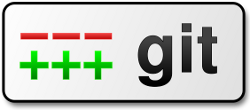
\includegraphics[width=40mm]{figuras/cap5/git.png}
 \caption{Logo de Git}
\end{figure}

En cada proyecto colaborativo hay muchos desarrolladores que necesitan hacer
muchos cambios, probar muchas alternativas de su código y sin embargo mantener
a todo el mundo informado y a su vez mantener una rama estable de desarrollo.
SVN no es demasiado eficiente a la hora de gestionar diferentes ramas de
desarrollo, ni al crearlas ni al unirlas.

Git soluciona este problema al fomentar los {\em commits} pequeños y una
herramienta de {\em merge} más eficiente, lo que facilita trabajar con ramas y
mantenerlas muy fácilmente. El trabajo con diferentes ramas de desarrollo y
una rama {\em master} siempre funcional, de fácil integración entre sí, facilita
el desarrollo considerablemente. Git fomenta este estilo de desarrollo.

Con su sistema de log y sus normas de estilo mejora el seguimiento de todos los
cambios, muy bien documentados, del código.

Por estas razones decidimos migrar la aplicación de SVN a Git cuando terminó el
CUSL. Esta migración nos obligó a buscar una nueva forja que nos proporcionara
este avanzado sistema de control de versiones. La elegida fue
Gitorious\footnote{\url{http://gitorious.org/}}, forja libre para proyectos
libres.

\begin{figure}[H]
 \centering
 
\includegraphics[width=40mm]{figuras/cap5/gitorious.png}
 \caption{Logo de Gitorious}
\end{figure}

\section*{Escenario de Simulación}

El escenario de simulación es la manera que tenemos de decirle a nuestro
simulador qué es lo que queremos simular precisamente. Dado que el simulador es
versátil y tiene capacidad de simular, en principio, cualquier lugar, hay que
definir una serie de parámetros de entrada.

En un escenario hemos de especificar cuál es el área con la que se va a
trabajar, cuáles son las entradas de agua y qué agentes humanos intervienen.
Aparte se definen también algunos parámetros técnicos como pueden ser los datos
de conexión a la base de datos de alturas.

Entrando en detalles los elementos de los que consta un escenario son:

\begin{description}
 \item[Nombre y descripción] Los escenarios se nombran para poder
identificarlos con facilidad, este nombre y descripción se muestra también en
los resultados de la simulación.
 \item[Fecha y hora] También se define la fecha y hora del comienzo de la
simulación, lo que permite localizar en el tiempo cada momento de la simulación.
 \item[Resolución temporal] Es necesario definir el tiempo transcurrido entre
dos estados de la simulación, tanto el tiempo simulado (en minutos) que
transcurre, como el tiempo de ejecución (en milisegundos) que se le concede a
la máquina -o máquinas- para simular un paso.
 \item[Área de simulación] El área viene definida por dos coordenadas
geográficas, la coordenada noroeste y la sureste del rectángulo -en realidad
no es un rectángulo si tenemos en cuenta la curvatura terrestre- que definen si
tomamos como diagonal el segmento que las une.
 \item[Resolución espacial] Uno de los parámetros más importantes que hay que
definir es la resolución espacial, tanto superficial como en altura. Hay que
especificar el tamaño de los hexágonos, lo que se hace a través del diámetro de
la circunferencia circunscrita en ellos -los hexágonos son regulares-. También
hay que definir la resolución espacial en altura, es decir, cómo se discretiza
la altura del terreno y del agua; se define como \begin{math}^1/_p\end{math}
metros de precisión donde {\em p} es el parámetro que aparece en el escenario.
 \item[Agentes Entorno] El número de agentes Entorno que se encargaran de
simular el escenario, el número adecuado depende de la cantidad de núcleos o
procesadores del que disponga la máquina donde se lleve a cabo la simulación.
 \item[Base de datos de alturas] En el escenario se incluyen también los datos
necesarios para realizar la conexión a la base de datos donde se almacenan la
elevación del terreno. Estos datos se obtienen de internet, pero se almacenan
localmente para agilizar simulaciones sucesivas en el mismo área.
 \item[Entradas de agua] A la hora de simular una inundación es básico simular
dónde y cuánta agua está entrando al sistema. Dichos datos se encuentran en el
escenario.
 \item[Peatones] La posición y características de los peatones, tales como su
distancia de visión, velocidad y objetivos -refugios que conocen de antemano-.
 \item[Frecuencia de actualización de resultados] Cada cuánto tiempo deben los
agentes Entorno enviar el estado de la simulación a los agentes encargados de
mostrar los resultados, así se define la finura de los resultados obtenidos.
\end{description}

Hay que destacar que los datos definidos en el escenario son los datos
iniciales de la simulación, y que muchos se traducen a agentes, como por
ejemplos las entradas de agua o las personas. Esto permite que en caliente se
puedan añadir, por ejemplo, nuevas fuentes de agua a la simulación, pues se
puede añadir agentes nuevos a una simulación en marcha.

\subsection*{Ejemplo de Escenario}

\lstinputlisting[caption=Escenario de ejemplo]{capitulo5/Ejemplo.scen}

Como se puede ver en el listado el formato de los ficheros escenario es {\em
clave=valor}, y para escribir un array -que son anidables, como se puede ver
también en el ejemplo- {\em clave=[elem,elem,elem...]}.

Lo primero que aparece es el {\em type}, es decir, el tipo de escenario del que
se trata. El valor es el nombre de la clase que hay que instanciar -que debe
heredar de {\em util.Scenario}-, por ahora sólo está implementado el caso de la
inundación, pero el escenario está preparado para múltiples tipos de desastres.

Es importante destacar que el orden en el que aparecen los elementos del
escenario en el fichero es irrelevante, cualquier orden es válido siempre que
aparezcan los elementos mínimos.

A continuación en el ejemplo aparecen el nombre ({\em name}), descripción ({\em
description}), fecha de inicio de la simulación ({\em date}) y hora inicial
({\em hour}).

Los dos siguientes elementos, {\em tick} y {\em realTick}, representan el
tiempo asignado a cada paso de la simulación. El primero se mide en
milisegundos y representa el tiempo de computación, es el que transcurre en
nuestro mundo; y el segundo se mide en minutos y representa cuanto tiempo ha
pasado dentro de la simulación.

{\em NW} y {\em SE} son dos arrays con las coordenadas geográficas de las dos
esquinas del área de simulación. Al igual que el resto de coordenadas que
aparecen en el escenario se escriben con el formato {\em [latitud,longitud]}.
{\em NW} hace referencia a la esquina noroeste, mientras que {\em SE}
referencia a la sureste.

{\em tileSize} corresponde al tamaño de los hexágonos, en metros, mientras que
{\em precision} define la resolución espacial en altura, en
\begin{math}^1/_{precision}\end{math} metros.

Seguido aparece el número de agentes {\bf Entorno}, con la clave {\em numEnvs}.
{\em randomTerrain} es un valor booleano que define si los entornos van a
utilizar datos reales de alturas, o van a generar terrenos aleatorios. Los dos
posibles valores que puede tomar son {\em True} y {\em False}, significando el
primero que el terreno simulado va a ser aleatorio.

A continuación vienen los datos necesarios para la conexión con la base de
datos de alturas. Todos comienzan por {\em DB}. {\em DBServer} es la url, ip,
nombre de fichero, etc, del servidor de base de datos. En este caso se trata de
un servidor que se encuentra en la misma máquina, y al que se accede por red
-de ahí las {\em //}-. {\em DBPort} es el puerto a usar para la conexión. {\em
DBUser} es el usuario con el que identificarse, y {\em DBPass} es la contraseña
en claro a utilizar. {\em DBDriver} especifica qué tipo de servidor se está
utilizando, en este caso se utiliza MySQL\footnote{\url{http://www.mysql.com/}}.
{\em DBDb} es el nombre de la base de datos donde se encuentra la tabla
{\bf Elevations}, dicha tabla está descrita en la sección donde se trata la
obtención de datos de alturas.

No todos los elementos {\em DB} son imprescindibles. Por ejemplo, si se utiliza
el servidor de base de datos de fichero
SQLite\footnote{\url{http://www.sqlite.org/}} no es necesario definir más que
{\em DBServer} y {\em DBDriver}.

Cada línea con la clave {\em waterSource} representa una entrada de agua
diferente al sistema, todas las entradas definidas en el fichero del escenario
se activan nada más comenzar la simulación. Para añadir fuentes de agua que
aparecen un tiempo después del comienzo de la simulación hay que añadir agentes
{\bf Entrada de Agua} en caliente. El array contiene los siguientes datos:
latitud, longitud y cantidad de agua que entra en cada tick medida en unidades
de altura de la simulación. El orden en que aparecen estos elementos es fijo.

Al igual que con las entradas de agua, puede haber múltiples líneas con la clave
{\em person}. Representan a agentes {\bf Peatón} en la simulación. Los
parámetros del array son, en orden, los siguientes: latitud, longitud,
distancia de visión en hexágonos, velocidad en hexágonos, número de clones y un
array de objetivos -con múltiples pares latitud y longitud, aunque en este caso
sólo hay un objetivo-. Todos estos parámetros serán discutidos en la sección de
los agentes {\bf Peatón}.

{\em updateTimeKML} y {\em updateTimeVisor} se miden ambos en milisegundos, y
hacen referencia al tiempo que transcurre entre que los agentes {\bf Entorno}
envían actualizaciones a los generadores de KML y a los visores respectivamente.

\subsection*{Generación de Escenarios}

Aunque es perfectamente posible escribir un fichero escenario con un editor de
textos, resulta más sencillo utilizar el script de lanzamiento de la simulación
para generar uno en un modo interactivo. Dicho modo se explica en detalle en la
sección dedicada al script de lanzamiento.

\section*{Agentes}

En esta sección se explicarán uno a uno todos los agentes que intervienen en la
simulación, y cómo se han implementado. Todos los agentes se encuentran en el
paquete, o en subpaquetes de éste, {\em agents}.

A continuación sigue un esquema con todos los agentes del simulador, los
comportamientos que utiliza cada agente, y flechas entre agentes que denotan
qué agentes se comunican entre sí.

\begin{figure}[H]
 \centering
 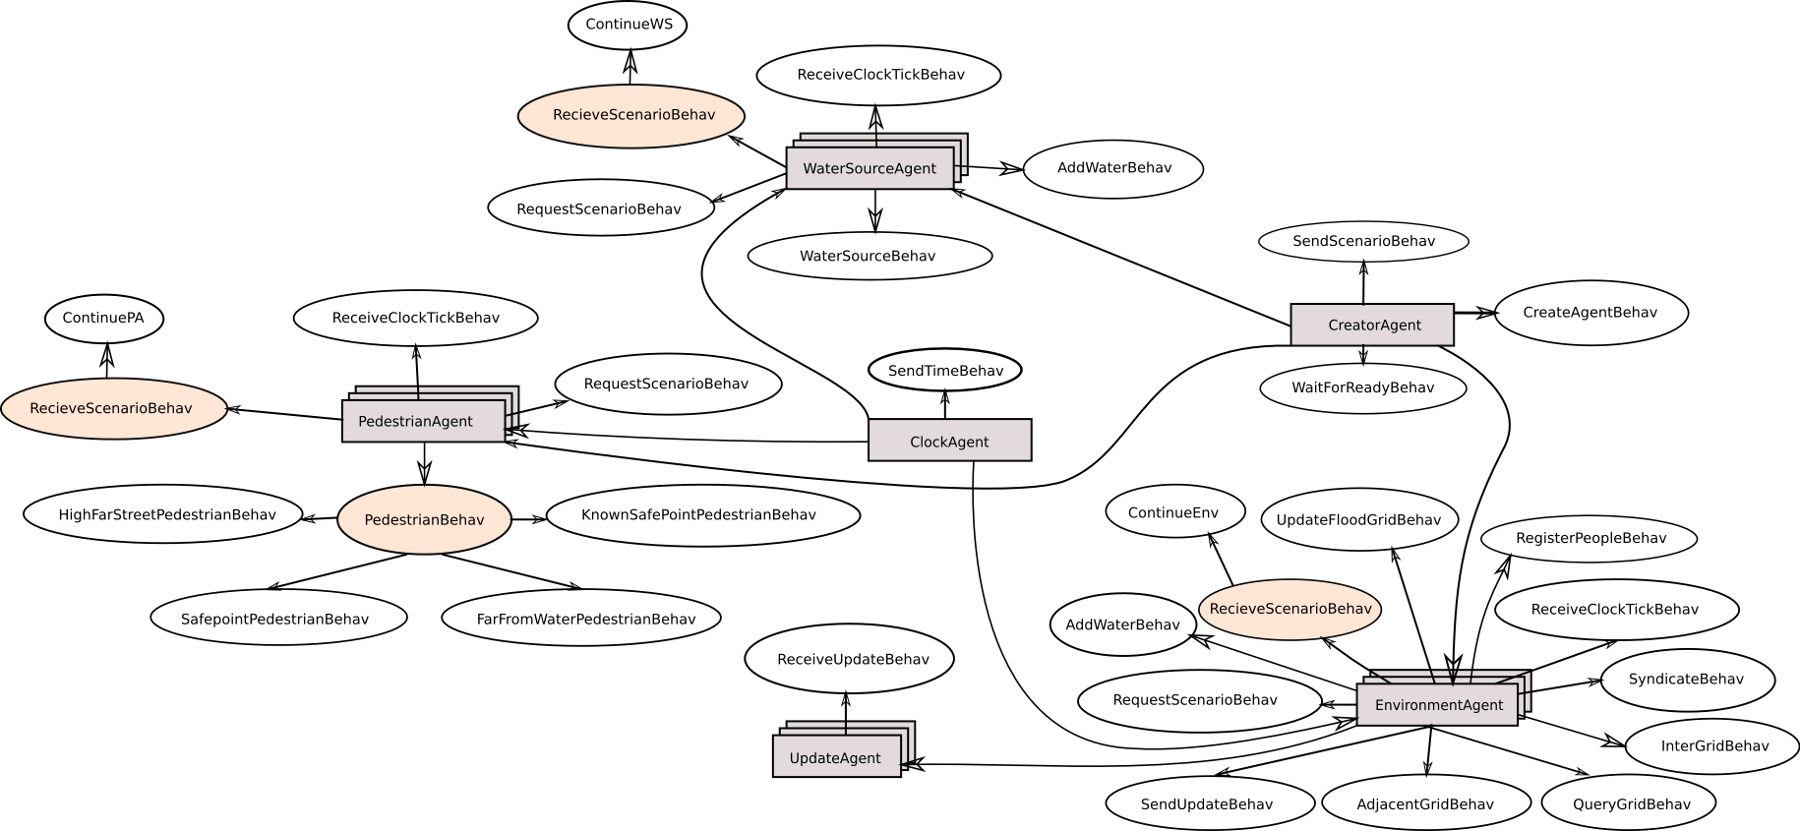
\includegraphics[height=100mm,angle=90]{figuras/cap5/agents.png}
 \caption{Esquema con todos los agentes}
\end{figure}

En programación con agentes lo habitual es que los agentes en sí no contengan
la lógica de su actividad, si no que tan sólo contienen el código de
inicialización y de finalización. Toda actividad que desarrolle el agente
durante su vida debe estar contenida en sus comportamientos, luego para que el
agente haga cualquier acción ha de añadírsele el comportamiento adecuado.

Para la programación de agentes utilizamos JADE, y JADE funciona mediante
herencia. Por ejemplo, para programar un agente hemos de extender la clase {\em
jade.core.Agent}. Y lo mismo para los comportamientos de los agentes, se
extiende la clase {\em jade.core.behaviours.Behaviour}. Una vez extendida la
clase correspondiente se implementan los métodos abstractos y se sobreescriben
los que se consideren necesarios.

Por ejemplo, en el caso de un agente, JADE proporciona una manera de
inicializarlo, que es sobreescribir el método {\em setup()}. JADE nos garantiza
que dicho método se ejecutará una única vez al crear el agente.

De la misma manera se trabaja con los comportamientos. Además JADE proporciona
múltiples clases de las que extender, estos comportamientos refinados -heredan
todos de {\em jade.core.behaviours.Behaviour}- facilitan la programación. Por
ejemplo, para un comportamiento que cree a otro agente lo habitual es sólo se
ejecute una vez, para ello se hereda directamente de {\em
jade.core.behaviours.OneShotBehaviour} y JADE nos asegura de que sólo se
ejecutará una vez.

A continuación pasamos a explicar los agentes del simulador. Por cada agente
hay un esquema de los comportamientos que utiliza, y en algunos de ellos -los
que inicien un diálogo con otros agentes- también hay un esquema de las
comunicaciones que mantienen.

Dichos esquemas de comunicación siguen el siguiente formato: A cada lado se
sitúa un agente, a la izquierda el que comienza el diálogo. Entre los agentes
hay flechas que representan mensajes, el sentido de la fecha denota al emisor y
al receptor. Sobre cada flecha va descrito, y en este orden, desde qué
comportamiento se envía, que comportamiento lo recibe, y de qué trata el
mensaje -tipo o contenido del mismo-. Obviamente el comportamiento que envía el
mensaje es del agente emisor, y el que recibe es del agente receptor.

\subsection*{Agente Creador}

La misión de este agente es la de crear al resto de agentes y lanzar la
simulación.

\begin{figure}[H]
 \centering
 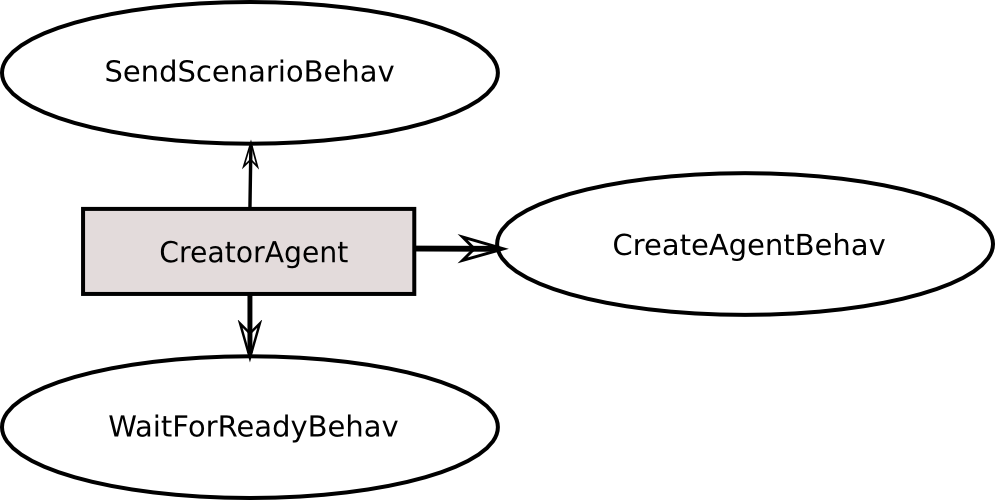
\includegraphics[width=100mm]{figuras/cap5/ag_creator.png}
 \caption{Agente Creador}
\end{figure}

Su ejecución consta de tres fases. En la primera procesa el fichero escenario y
crea a los agentes {\em Entorno}, a través del comportamiento {\em
CreateAgentBehav}, que es el comportamiento utilizado para crear agentes y que
se encuentra en el paquete {\em behaviours}. El agente se queda esperando a que
los agentes {\bf Entorno} terminen de inicializarse, para ello utiliza el
comportamiento {\em WaitForReadyBehav}, del mismo paquete.

Una vez listos, el agente {\bf Creador} pasa a la segunda fase en donde crea al
resto de agentes: {\bf Entradas de Agua}, {\bf Peatones}, etc, todo según se
describa en el escenario. Es necesario esperar a que se inicialicen los
entornos, dado que es un proceso lento (han de obtener las alturas y las
calles) y el resto de agentes los necesitan preparados pues les preguntan cosas.
Por último crea al agente {\bf Reloj} dando comienzo así a la simulación.

En la tercera y última fase, el {\bf Creador} se queda inactivo a la espera de
mensajes que soliciten el objeto escenario, enviándoselo a los agentes que
manden dichos mensajes. Esta actividad la realiza a través del comportamiento
{\em SendScenarioBehav}.

Este último comportamiento actúa como servidor del objeto escenario, y se
implementa mediante un {\em CyclicBehaviour} de JADE.

\subsection*{Agente Reloj}

Este agente apareció en nuestro sistema considerablemente tarde, por lo que
tuvimos que hacer bastantes cambios para incluirlo. Nació de la necesidad de
sincronizar los diferentes agentes de la simulación.

Esta necesidad quedó patente cuando generábamos ficheros KML con datos de
múltiples entornos. Al visualizar estos ficheros veíamos cómo zonas de la
simulación se adelantaban a otras, efecto que no se apreciaba fuera del KML
porque era consecuencia del desajuste de la fecha y hora de los entornos, no
porque no se hubiesen simulado al mismo tiempo.

En un primer momento implementamos un sistema que escogía arbitrariamente a un
agente {\bf Entorno} y lo designaba como reloj, el encargado de esta selección
era el agente {\bf Creador} -porque se trata del único agente del que no hay
puede haber múltiples copias en una simulación-. Los agentes {\bf Entorno} se
proponían como relojes cuando recibían agua de una {\bf Entrada de Agua}, pues
usaban éstas como forma de medir el tiempo. El {\bf Creador} escogía al primero
de ellos y éste se encarga de avisar al resto cada vez que se actualizaba el
reloj. Este sistema se demostró muy poco eficaz y provocó la aparición de los
mencionados desajustes.

La solución fue la creación del agente {\bf Reloj} y el establecimiento de un
tick de simulación. Los agentes sometidos a ese tick son todos aquellos cuya
tarea depende del tiempo simulado, que son los {\bf Entornos}, {\bf Entradas
de Agua} y {\bf Peatones}.

\begin{figure}[H]
 \centering
 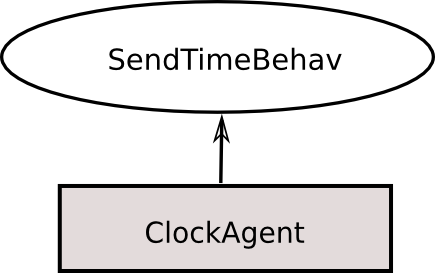
\includegraphics[width=50mm]{figuras/cap5/ag_clock.png}
 \caption{Agente Reloj}
\end{figure}

Este agente tiene un comportamiento de tipo {\em
jade.core.behaviours.TickerBehaviour}, que se ejecuta periódicamente según un
intervalo definido en el escenario. Cada vez que se ejecuta manda un mensaje a
los agentes comentados anteriormente, dando lugar a un nuevo paso de la
simulación. En dicho mensaje manda la fecha y hora dentro de la simulación,
correspondiente a ese paso. Todos los agentes que reciben estos mensajes lo
hacen a través del comportamiento {\em behaviours.ReceiveClockTickBehav}.

De esta forma se solucionan los problemas de sincronización entre agentes, se
eliminan los desajustes del KML, se soluciona el problema del cálculo de la
velocidad de los peatones e, incluso, se mejora la escalabilidad del sistema,
dado que aumentando el periodo permitimos que el simulador corra en máquinas
menos potentes.

Esta técnica de sincronización se utiliza mucho cuando se trabaja con JADE y
hay que sincronizar los agentes, pues JADE es de naturaleza asíncrona.

\begin{figure}[H]
 \centering
 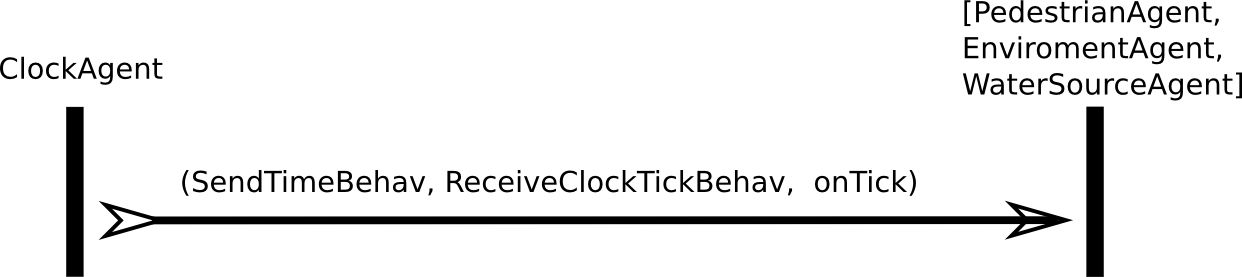
\includegraphics[width=120mm]{figuras/cap5/com_clock.png}
 \caption{Comunicaciones del agente Reloj}
\end{figure}

\subsection*{Agentes Entorno}

Los agentes {\em Entorno} son sin duda los más complejos y los más importantes
de cuantos forman la simulación. Su papel es manejar y mantener la información
del terreno simulado. Se encarga de obtener los datos de altura y calles, de
mover el agua de la inundación, de responder a los {\bf Peatones}, de enviar el
estado de la simulación a los agentes {\bf Actualización}, etc.

Durante su inicialización este agente obtiene los datos necesarios del terreno
que le toca simular, o de una base de datos o bien de un servicio web. La manera
en la que se descargan estos datos será explicada en la sección correspondiente.

Una vez inicializado el terreno, el agente crea y añade sus comportamientos, y
se registra en el servicio de ``páginas amarillas'' de JADE -{\em Directory
Facilitator} (DF)- para que el resto de agentes pueda encontrarlo. Por último
avisa al agente {\bf Creador} de que está listo para comenzar la simulación.

Para representar este terreno optamos por una maya hexagonal, que manejamos
mediante la clase {\em util.HexagonalGrid}. Cada agente {\bf Entorno} posee una
instancia de dicha clase con los datos de su trozo de simulación. Como es el
entorno el que posee los datos del terreno, proporciona también servicios de
consulta de dicha información al resto de agentes. Dichos servicios se
implementan mediante comportamientos del tipo {\em
jade.core.behaviours.CyclicBehaviour}, en particular se trata de los
comportamientos {\em behaviours.AdjacentsGridBehav} y {\em
behaviours.QueryGridBehav}.

\begin{figure}[H]
 \centering
 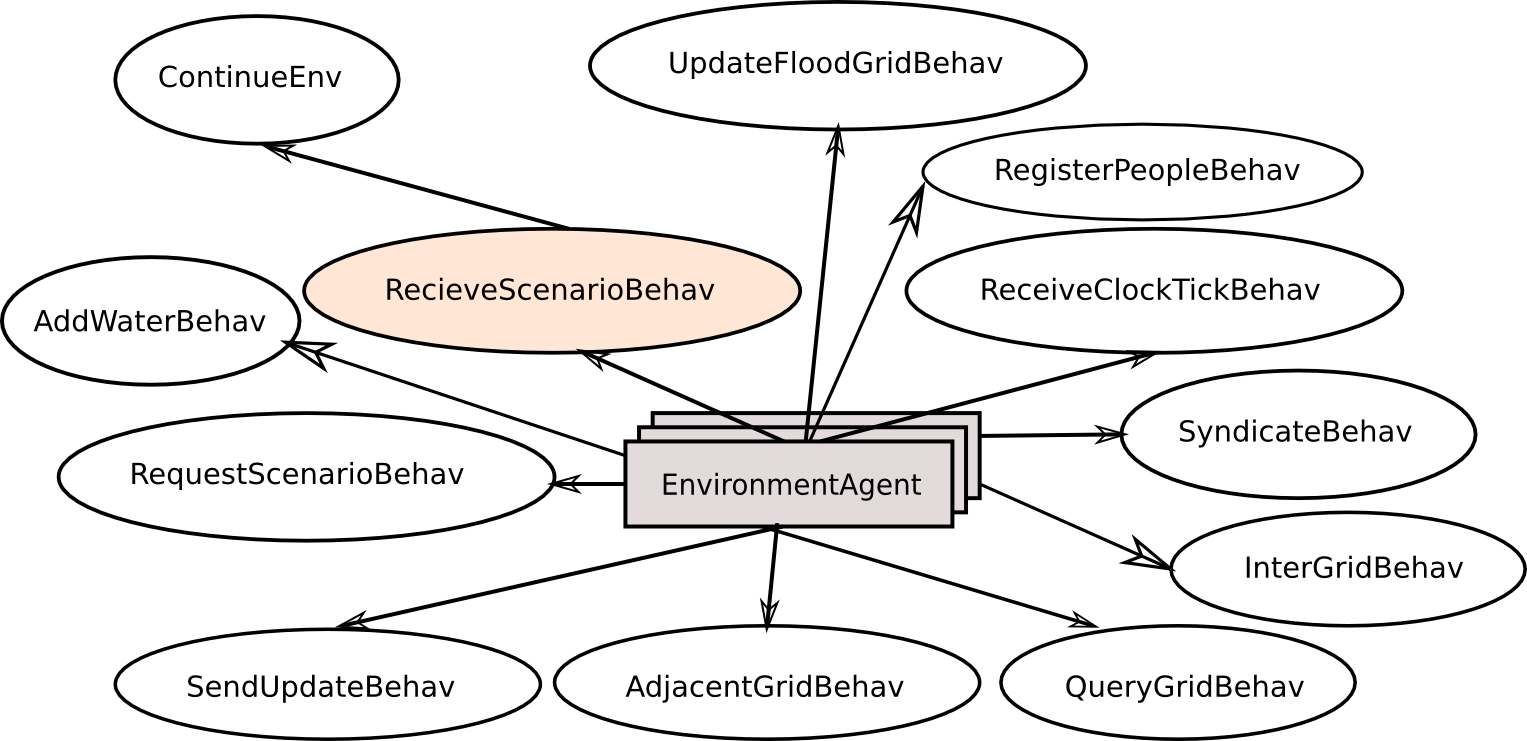
\includegraphics[width=130mm]{figuras/cap5/ag_environment.png}
 \caption{Agente Entorno}
\end{figure}

Los comportamientos {\em behaviours.flood.AddWaterBehav}, de tipo cíclico, y el
{\em behaviours.flood.UpdateFloodGridBehav}, de tipo periódico, son propios de
inundaciones. El primero recibe y procesa los mensajes de las entradas de agua,
añadiendo más agua a la simulación si fuera necesario -si resulta que la fuente
de agua no está a un nivel superior que el agua que la rodea, el nuevo agua se
desestima-. El segundo es el encargado de mover el agua por el terreno.

{\em behaviours.InterGridBehav} es un comportamiento que se encarga de la
comunicación entre {\bf Entornos}. Cuando, por ejemplo, el agua llega al borde
del terreno simulado por el agente, busca al {\bf Entorno} que simula el trozo
correspondiente y le avisa de que le llega agua, si es que existe tal {\bf
Entorno}.

El comportamiento {\em behaviours.SyndicateBehav} es el comportamiento
utilizado por los agentes {\bf Actualización} para darse de alta o baja en la
recepción del estado de la simulación.

{\em behaviours.people.RegisterPeopleBehav} es el comportamiento con el que se
comunican los {\bf Peatones} para avisar al entorno de su posición y salud.

\begin{figure}[H]
 \centering
 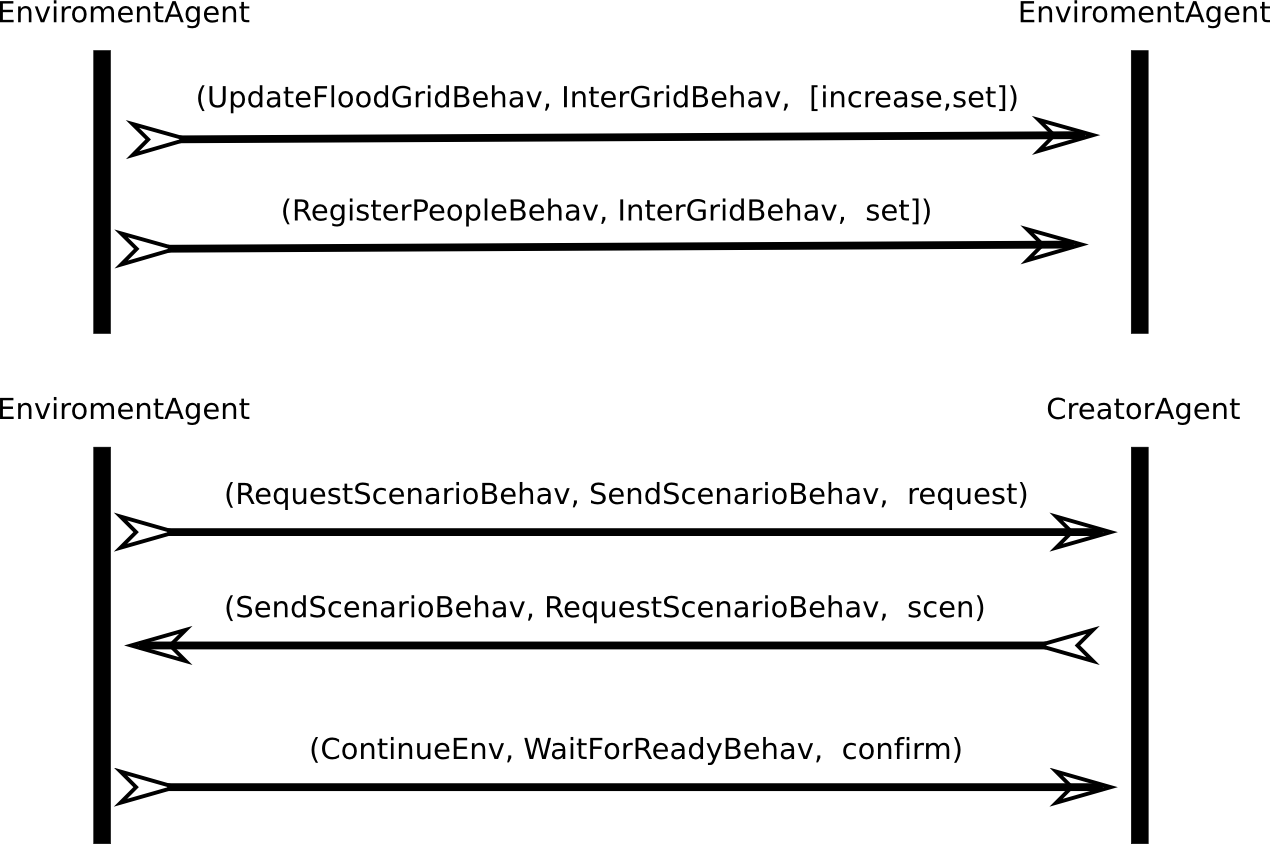
\includegraphics[width=120mm]{figuras/cap5/com_environment.png}
 \caption{Comunicaciones del agente Entorno}
\end{figure}

\subsubsection*{Casillas Adyacentes y Múltiples Entornos}

El {\bf Entorno} recibe muchas peticiones, normalmente de los {\bf Peatones},
solicitando las casillas adyacentes a una dada. El agente consulta su maya
hexagonal y devuelve las casillas pedidas.

El único problema es que un {\bf Entorno} sólo conoce lo que ocurre en el
terreno que simula, pero no los datos del resto de {\bf Entornos}. Para los
{\bf Peatones} esto es un problema, pues para ellos el que se simule con
múltiples {\bf Entornos} debería ser transparente. Esto significa que las
fronteras que separan los trozos de terreno de los diferentes agentes {\bf
Entorno} suponen una barrera a la visión de los {\bf Peatones}, lo cual no
tiene ningún sentido.

Para solucionar dicho problema tuvimos que refinar el comportamiento {\em
AdjacentsGridBehav}, y hacer que cuando detectase que la casilla de la que se
solicitan los adyacentes está más cerca del borde del terreno que la distancia
de visión pedida, entonces solicitase los adyacentes restantes a los agentes
{\bf Entorno} correspondientes.

Es decir, que cuando un agente {\bf Peatón} solicita los hexágonos adyacentes a
uno dado a un {\bf Entorno} concreto, puede estar involucrando a más agentes en
el proceso pero sin saberlo. Para los {\bf Peatones} este proceso es del todo
transparente.

\subsubsection{Movimiento del Agua}\label{waterMovement}

Dadas las limitaciones vistas en el \hyperref[cap2]{capítulo 2}, y sobre todo
dada nuestra intención de crear un modelo sencillo y abarcable, hemos
implementado un relativamente sencillo comportamiento para simular el
movimiento del agua. Dicho comportamiento es {\em UpdateFloodGridBehav}.

El funcionamiento del algoritmo es el siguiente:

\begin{enumerate}
 \item Se solicitan a la maya hexagonal las casillas cuyo nivel de agua ha sido
 modificado desde la última vez que se ejecutó el algoritmo.
 \item Se recorren dichas casillas, y se consulta el valor del agua y terreno
 de las casillas inmediatamente adyacentes.
 \item Si se encuentran casillas adyacentes más bajas entonces se mueve agua a
 dichas casillas -se mueve la mitad de la diferencia en altura, es decir, se
 iguala el nivel-. Si se encuentran casillas más altas se trae agua de dichas
 casillas.
 \item Todas las casillas cuyo nivel de agua haya sido afectado se marcan como
 modificadas, y serán revisadas por la siguiente pasada del algoritmo.
\end{enumerate}

Para el funcionamiento de este algoritmo cuando se simula en múltiples {\bf
Entornos} se hizo necesario incluir un borde exterior extra o corona a las mayas
hexagonales. Esta corona es del ancho de una casilla y mantiene el valor del
terreno y nivel de agua, aunque no se muestra en los visores. La utilidad de
esta corona es saber cuándo se debe pasar agua, y cuánta, a otros {\bf
Entornos}.

Cuando un {\bf Entorno} decide mover agua de una de sus casillas a una de la
corona comprueba a qué {\bf Entorno} pertenece dicha casilla. Si lo encuentra
le avisa de que ha añadido agua a la casilla. Si no lo encuentra es que es una
casilla fuera de la simulación con lo que el agua se pierde. El simulador
desconoce qué le ocurre a todo el agua que se sale de la simulación, por lo que
los bordes exteriores, no las fronteras entre {\bf Entornos}, son sumideros por
los que desaparece agua de la simulación. La cantidad de agua que desaparece
viene determinada por la altura del terreno, otra utilidad de la corona.

También ocurre que cuando un {\bf Entorno} modifica el nivel de agua de una
casilla del borde inmediatamente interior a la corona -es decir, el borde
exterior de su área de simulación- debe avisar del nuevo nivel al agente que
tenga esa casilla como corona, si es que lo hay.

Para manejar toda esta comunicación entre {\bf Entornos} creamos el
comportamiento {\em InterGridBehav}.

Como anécdota cabe comentar que en una primerísima versión del simulador,
cuando estábamos aún diseñándolo y haciendo pruebas, optamos por agentificar el
agua. De esta forma cada ``gota'' de agua era un agente que recorría el terreno
y escogía donde quedarse, inundando la casilla. El sistema funcionaba pero muy
poco escalable, dado que la cantidad de agentes agua era abrumadora. Lo
desechamos rápidamente y comenzamos el diseño del sistema actual.

\subsection*{Agentes Entrada de Agua}

Este tipo de agente es de lo más sencillo. Son agentes para nada inteligentes,
cuya única misión es enviar un mensaje al {\bf Entorno} correspondiente en cada
paso de la simulación avisándole de la cantidad de agua que debe añadir.

\begin{figure}[H]
 \centering
 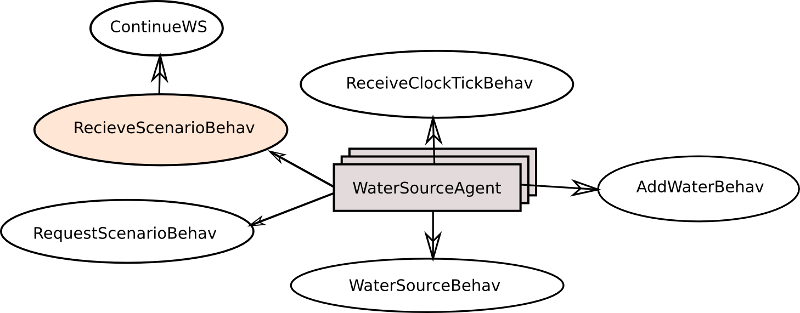
\includegraphics[width=120mm]{figuras/cap5/ag_water_source.png}
 \caption{Agente Entrada de Agua}
\end{figure}

En su inicialización el agente busca su {\bf Entorno}, para ello necesita
conocer el escenario de simulación que solicita al agente {\bf Creador}.
Consultando las coordenadas geográficas donde está situado y el escenario
descubre en qué trozo del terreno ha caído. A partir de ahí se limita a mandar
un mensaje en cada tick del {\bf Reloj}.

\begin{figure}[H]
 \centering
 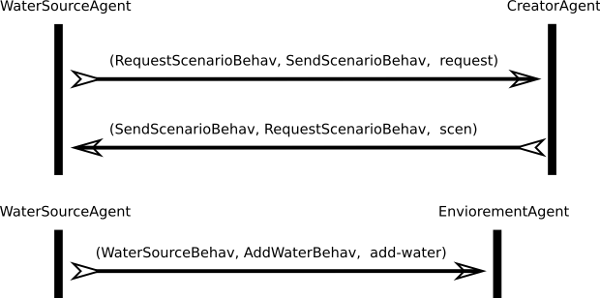
\includegraphics[width=120mm]{figuras/cap5/com_water_source.png}
 \caption{Comunicaciones del agente Entrada de Agua}
\end{figure}

\subsection*{Agentes Peatón}

Durante la inicialización estos agentes averiguan cuál es el {\bf Entorno} cuyo
terreno contiene su coordenada inicial, para ello utilizan el escenario que
solicitan al agente {\bf Creador}. Una vez inicializados comienzan a moverse
por el terreno tratando de salvarse de la inundación.

\begin{figure}[H]
 \centering
 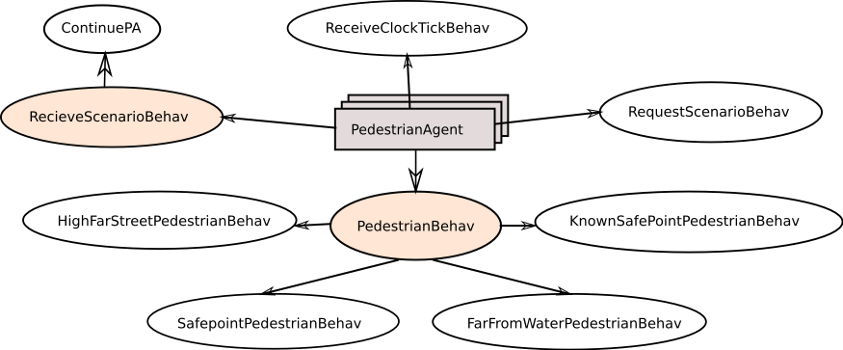
\includegraphics[width=135mm]{figuras/cap5/ag_pedestrian.png}
 \caption{Agente Peatón}
\end{figure}

Como hemos visto en el escenario de simulación, los agentes {\bf Peatón}
reciben una serie de parámetros de entrada. A saber:

\begin{description}
 \item[Posición inicial] Dado en coordenadas geográficas latitud,longitud.
 \item[Distancia de visión] Medida en hexágonos, representa cuantos hexágonos
 es capaz de ver el peatón en línea recta. Se utiliza a la hora de solicitar
 casillas adyacentes a la posición en ese momento.
 \item[Velocidad] La cantidad de hexágonos que la persona es capaz de recorrer
 en un único paso de simulación.
 \item[Objetivos] Coordenadas geográficas de los refugios que el {\bf Peatón}
 conozca desde el principio. Pueden ser más de uno, uno, o directamente ninguno.
\end{description}

El comportamiento base de todos los {\bf Peatones} funciona de la siguiente
manera:

\begin{enumerate}
 \item Solicitar casillas adyacentes según distancia de visión al {\bf Entorno}.
 \item Recibir casillas y escoger a cuál moverse.
 \item Si se ha escogido casilla, avisar al {\bf Entorno} de la nueva posición.
 Si no, volver al paso 1 sin moverse de la posición.
\end{enumerate}

Es en el segundo paso donde reside toda la complejidad, justo a la hora de
escoger a qué casilla moverse. Para facilitar la implementación de diferentes
comportamientos hemos implementado un comportamiento base abstracto, {\em
behaviours.people.PedestrianBehav}, del que heredar. Heredando de dicho
comportamiento lo único que hay que hacer es implementar un método {\em
choose(Set$<$Point$>$ adjacents)} que es dónde se escoge la casilla a la que
moverse.

Nosotros hemos ido perfeccionando y refinando el comportamiento de las
personas, habiendo desarrollado los siguientes -todos ellos en el paquete {\em
behaviours.people.flood}-:

\begin{description}
 \item[FarFromWaterPedestrianBehav] El primer y más simple de los
 comportamientos, el agente tan sólo escoge la casilla más alejada del agua
 que alcanzaba a ver.
 \item[HighFarStreetPedestrianBehav] Esta segunda aproximación es un poco más
 sofisticada pues tiene en cuenta también la altura de las casillas. Se pondera
 y se asigna una puntuación a cada casilla según lo alejada del agua que esté,
 y lo alta que sea. Escoge la casilla con mejor puntuación.
 \item[SafepointPedestrianBehav] Este comportamiento ya es bastante más
 complejo. Los agentes se desplazan según una dirección aleatoria, pero
 manteniéndola. De esta forma van recorriendo las calles de la ciudad, y
 cuando llegan a cruces de calles existe la posibilidad de que cambien de
 dirección y comiencen a recorrer alguna bocacalle. Cuando ven agua escogen la
 dirección contraria y huyen de ella, y cuando ven un refugio corren a él y se
 ponen a salvo.
 \item[KnownSafepointPedestrianBehav] La última evolución del comportamiento
 implica el conocimiento a priori por parte de los agentes de la posición de
 algún refugio. El agente trata de alcanzar algunos de los refugios que conoce,
 aunque si por el camino encuentra algún refugio se recoge en él. En caso de no
 tener objetivos o ser estos inaccesibles -la inundación le ha cortado el paso,
 por ejemplo- se comporta como el {\em SafepointPedestrianBehav}.
\end{description}

En este último comportamiento, el {\em KnownSafepointPedestrianBehav}, fue
necesario dotar al agente de memoria. Un problema que encontramos cuando
probábamos el comportamiento es que en ocasiones el agente se quedaba atascado
intentando atravesar edificios. Y es que la casilla más cercana al refugio
podía coincidir con su posición actual, dado que el cálculo de la distancia no
tiene en cuenta los edificios ni las calles. Al dotar de memoria al agente, y
penalizar severamente el moverse a casillas por las que acaba de pasar,
solucionó el problema. El agente prefiere dar un rodeo y alejarse temporalmente
del refugio a volver sobre sus pasos o quedarse quieto.

\begin{figure}[H]
 \centering
 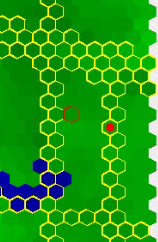
\includegraphics[width=35mm]{figuras/cap5/atasco.png}
 \caption{Peatón atascado}
\end{figure}

Como se puede apreciar en la imagen la casilla en la que se encuentra el peatón
-el punto rojo- es la más cercana al refugio -hexágono de borde rojo-. Esto
provocaba que el agente se quedase quieto u oscilase alrededor de dicha casilla.

Cabe destacar que no se han tenido en cuenta ni la capacidad de las calles ni
de los refugios, el número de personas que puede haber en una casilla es
ilimitado.

\begin{figure}[H]
 \centering
 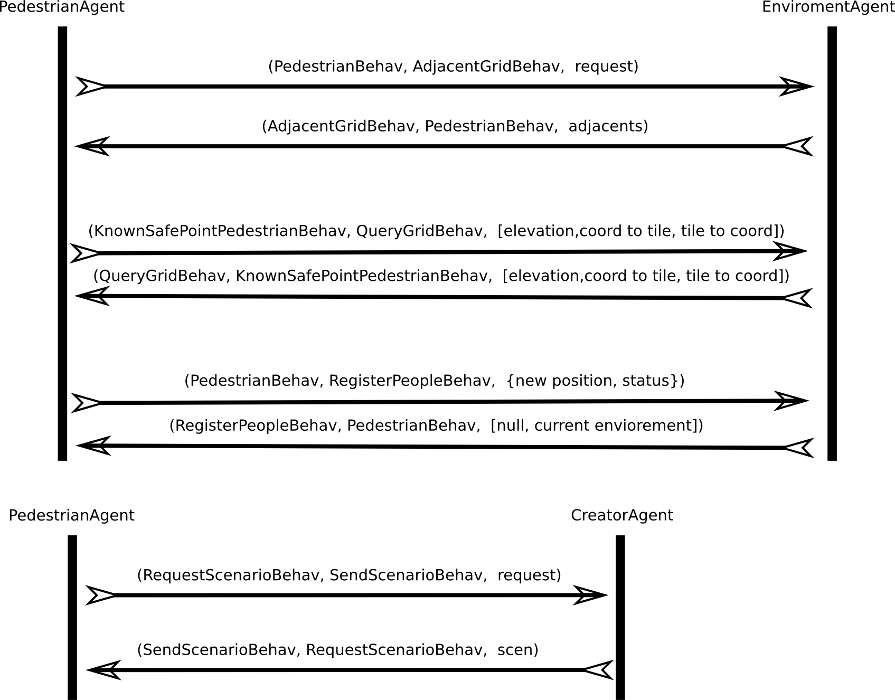
\includegraphics[width=135mm]{figuras/cap5/com_pedestrian.png}
 \caption{Comunicaciones del agente Peatón}
\end{figure}

\subsection*{Agentes Actualización}

Estos agentes nos permiten sacar información de la simulación. Durante su
inicialización lo que hacen es subscribirse a los agentes {\bf Entorno} que se
le pasen por parámetros.

Los {\bf Entornos} le enviarán periódicamente un objeto de tipo {\em
util.Snapshot} con el estado de la simulación en ese momento.

\begin{figure}[H]
 \centering
 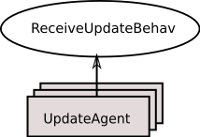
\includegraphics[width=50mm]{figuras/cap5/ag_update.png}
 \caption{Agente Actualización}
\end{figure}

Todos los agentes {\bf Actualización} tiene un objeto cliente, que debe
implementar la interfaz {\em util.Updatable}. Son estos objetos los que
procesan los {\em snapshots} y producen algún resultado.

Por ejemplo, los generadores KML o los extractores de estadísticas, interactúan
con la simulación a través de un agente {\bf Actualización}, y ambos
implementan {\em Updatable}. Se pueden escribir nuevos clientes para estos
agentes sin tener que modificarlos, dado que reciben por parámetros el nombre
de la clase del cliente de la que crean la instancia mediante reflexión.

\begin{figure}[H]
 \centering
 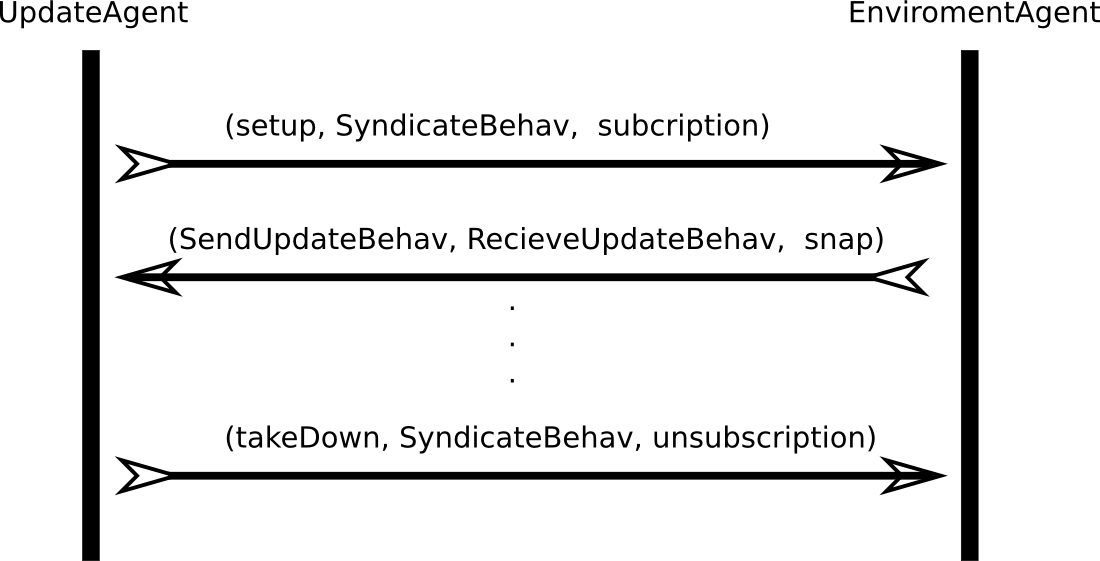
\includegraphics[width=100mm]{figuras/cap5/com_update.png}
 \caption{Comunicaciones del agente Actualización}
\end{figure}

\section*{Maya Hexagonal}

Sobre la rejilla es donde se van a realizar todos los cálculos de la simulación,
por lo tanto dispone de todos los métodos para manipular y obtener la
información contenida en ella. También contiene funcionalidad básica como
obtener todos los adyacentes a un punto, o calcular la distancia que separa a
dos casillas. La implementación de la maya hexagonal se encuentra en la clase
{\em util.HexagonalGrid}.

La manera de almacenar la información es a través de matrices cuadradas, los
métodos de acceso y cálculo de adyacentes la hacen parecer una maya hexagonal a
quien los usa. Todas las matrices almacenan datos de tipo {\em short}, pues no
es necesario un rango mayor y así se ahorra memoria. Todas las matrices son de
la misma dimensión.

\subsection*{Matriz de Alturas}

El rango del tipo básico {\em short} en Java va desde -32768 hasta 32767, y
dependiendo de la precisión en altura que se esté utilizando el rango en metros
será menor o mayor que éste.

\subsection*{Matriz de Agua}

Para el caso de inundación se añade esta matriz, que a diferencia de la matriz
de alturas, sólo almacena valores positivos -no tiene sentido un nivel de agua
negativo-. Los valores de esta matriz cambiarán a lo largo de la simulación,
otra diferencia con respecto a la matriz de alturas.

Sumando los valores de una casilla en las matrices de alturas y agua se obtiene
la altura total del terreno en ese punto.

\subsection*{Matriz de Calles}

Esta matriz no se modifica una vez rellena, y almacena valores clave que definen
el tipo de casilla del que se trata. Valores del tipo ``calle'', ``avenida'',
``autovía'', ``hotel'', ``río'', etc.

Gracias a estos valores los agentes tienen una representación de las
construcciones y calles que los rodean.

\subsubsection*{Tipos de Calles}

Para saber en qué tipo de calle nos encontramos nos ayudamos de la información
de OSM, que viene categorizada en grupos, tales como ``carreteras``, ''puntos
de interés``, ``vías de agua``, etc. A cada grupo le asignamos un rango de
valores, teniendo en cuenta el número de subgrupos que tiene. Por ejemplo, el
grupo ''carreteras`` tiene múltiples subgrupos, como pueden ser ''calle``,
''avenida``, ''autovía``, etc.

Estos valores los identificamos por medio de constantes globales; y se
comparan mediante funciones estáticas, que nos devuelven el tipo concreto o los
valores padre -para los subgrupos-.

\subsubsection*{Prioridad de la Información}

Ocurre que en ocasiones varios elementos caen en la misma casilla, pues están
muy cercanos geográficamente y les corresponde el mismo hexágono. Pero en cada
casilla sólo podemos almacenar un valor, por lo que rellenamos la matriz de
forma que se sobreescribe el valor que hubiera si el nuevo valor es mayor que el
viejo. Así nos aseguramos que la información que consideramos más prioritaria
-de mayor valor- permanezca en la matriz.

\subsubsection*{Intersecciones}

A veces es útil, sobre todo en el caso de las calles, saber cuando se cruzan
dos o más elementos. Para ello, a la hora de sobreescribir valores, si nos
encontramos con que había un valor igual al que nosotros queremos insertar,
incrementamos en una unidad el valor que hubiese -haciéndolo impar-.

Obviamente para que este sistema funcione, los valores que insertemos
normalmente en la matriz -cuando no se sobreescribe ningún valor- tienen que ser
todos pares. Así si el valor de una casilla es impar sabemos que en ese punto
hay una intersección de dos elementos.

\subsection*{Coronas}

Como se comentó en la sección del \hyperref[waterMovement]{movimiento del agua}
de los agentes {\bf Entorno}, las mayas hexagonales disponen de una corona, o
borde extra, de casillas. Esta corona -de ancho un único hexágono- contiene los
datos de altura y nivel de agua de casillas que pueden pertenecer a {\bf
Entornos} vecinos.

La necesidad de establecer estas coronas viene de poder efectuar las
simulaciones en más de un {\bf Entorno}, pues teníamos que crear un sistema para
actualizar valores de casillas en los {\bf Entornos} vecinos.

De esta forma, cuando se modifica la información de una corona, el agente {\bf
Entorno} busca qué otro agente {\bf Entorno} -si que lo hay- posee dicha
casilla y le avisa de la actualización realizada. Así se mantiene la coherencia
entre {\bf Entornos} y el paso de uno a otro se vuelve transparente para el
resto de agentes.

\subsection*{Coordenada a Casilla, y Viceversa} \label{coordToCasilla}

El paso de coordenada geográfica a coordenada en la maya, y viceversa, es un
problema complejo que ha requerido un considerable esfuerzo. Hay que tener en
cuenta que la maya es hexagonal, y que la tierra no es plana.

\subsubsection*{Incrementos} \label{incrementos}

Para poder convertir la posición de una casilla a una determinada coordenada
geográfica hemos optado por la técnica de los incrementos, en vez de complicados
cálculos trigonométricos terrestres.

La técnica consiste en hallar la diferencia en grados decimales entre los
extremos del mapa, y dividirla entre el número de filas y columnas. Con esto
obtenemos el incremento en latitud o longitud que hay entre cada casilla de
nuestra rejilla.

Debido a la forma de la rejilla hexagonal tenemos que tener en cuenta que las
filas impares tienen un offset de \begin{math}^1/_2\end{math} de incremento de
latitud, y que las columnas tienen un incremento de \begin{math}^3/_4\end{math}
de incremento de la longitud.

De esta forma tan sencilla podemos hacer las conversiones de ''casilla a
coordenada``.

\subsubsection*{Discretización}

El problema de ''coordenada a casilla'' es un poco más complejo, puesto que al
trabajar con una coordenada tenemos que aproximar a una casilla en concreto
-la coordenada, muy probablemente, no va a coincidir con el centro de ningún
hexágono-.

Para ello primero realizamos una aproximación a grandes rasgos intentando
averiguar la casilla, sin embargo la forma de las casillas es hexagonal, por lo
que hay que asegurarse de que la casilla sea la correcta. Se refina la casilla
escogida calculando la distancia al centro de los hexágonos, escogiendo siempre
la más cercana. Pero como las casillas son hexagonales, no circulares, siempre
existe una posibilidad de error.

De esta forma perdemos un poco de información, pero los errores cometidos por
este sistema no superan el \begin{math}0.7\%\end{math}.

\section*{Especialización: Múltiples Desastres}

Siguiendo el estilo de JADE, con el que se trabaja a través de los mecanismos
de herencia de Java, hemos diseñado nuestro simulador para que se pueda
extender a múltiples desastres mediante herencia.

Por ejemplo, clases como {\em Scenario} o {\em HexagonalGrid} no se pueden
instanciar directamente, si no que hay que utilizar las clases hijas {\em
FloodScenario} y {\em FloodHexagonalGrid}. De la misma manera, implementando
nuevas clases hijas que sobreescriban de otra manera los métodos se podría dar
soporte a nuevos tipos de desastres naturales.

Las clases padres dan funcionalidad básica y común a todos los desastres. Por
ejemplo, {\em HexagonalGrid} mantiene las matrices de alturas y de calles,
mientras que es {\em FloodHexagonalGrid} la que añade la matriz de agua.

\section*{Elevación del Terreno}

Para la obtención de alturas utilizamos servicios de información en la red. Por
desgracia la obtención de estos datos puede resultar lenta, por lo que se hizo
necesario implementar una caché de alturas.

\subsection*{Caché de Alturas}

Obtener todas las alturas de todas las casillas cada vez que necesitemos
simular un escenario no es viable. La solución que nosotros implementamos es
almacenar en local los datos para utilizarlos de nuevo en posteriores
simulaciones, o incluso para poder reutilizarlos en otras máquinas.

El almacenamiento se realiza en un servidor de base de datos, al que se accede
a través de JDBC\footnote{Java Database Connectivity:
\url{http://java.sun.com/products/jdbc/overview.html}}. Por ahora están
soportados por el simulador los servidores MySQL, PostgreSQL y SQLite, pero
sería muy sencillo incluir más servidores siempre que haya un driver para JDBC.

La base de datos sólo contiene una tabla, de nombre Elevations, con tres campos:

\begin{center}
\begin{tabular}{ | l | c | r | }
\hline
{\bf Campo} & {\bf Tipo de datos} \\ \hline
Lat & DOUBLE \\ \hline
Long & DOUBLE \\ \hline
Elev & DOUBLE \\ \hline
\end{tabular}
\end{center}

El simulador intenta obtener los datos de la base de datos local, para ello
busca las alturas de las coordenadas que caigan dentro del hexágono y hace la
media de los resultados, y en caso de que no haya ninguna altura en la base de
datos la descarga del servicio web y la añade.

Es posible añadir nuevas fuentes de datos de alturas al simulador. Para ello es
necesario implementar el cliente del nuevo servicio cumpliendo con la interfaz
{\em elevation.ElevationService}.

\section*{Open Street Maps}

OSM permite la descarga de ficheros XML que contienen toda la información de
sobre las calles, puntos de interés, etc, contenidas en unas coordenadas
determinadas.

La {\em url} para descargar estos ficheros se compone de la siguiente manera: 
{\em dirección base + coordenada suroeste + coordenada noreste}. El fichero
descargado tendrá el mismo nombre que la petición.

\subsection*{Parsear XML}

La información viene codificada en un fichero XML siguiendo el estándar de OSM.
Para poder extraer la información es necesario parsear el fichero. Para ello
utilizamos JAXB\footnote{Java Architecture for XML Binding: 
\url{https://jaxb.dev.java.net/}}, que es una librería para recorrer ficheros
XML. 

Mientras realizamos el recorrido del fichero hay que identificar la información
de las etiquetas y almacenarla en nuestra estructura de datos para poder
utilizarla de una forma mas cómoda. El diseño de las clases que hemos
implementado para almacenar la información es muy parecido a la jerarquía de
información que sigue OSM.

La clase principal es {\em OsmMap}, que contiene toda la información que nos da
OSM. {\em OsmWay} es para la etiqueta {\em way} (camino o vía) de OSM, y {\em
OsmMember} para los caminos compuestos. {\em OsmRelation} para los ríos y
parques, y {\em OsmNode} para los puntos simples y puntos de interés. Para
almacenar la información extra creamos {\em OsmTag}.

\subsubsection*{Filtro de Información}

{\em OsmTag} contiene dos atributos principales, clave y valor. Nos valemos de
estos dos atributos para almacenar la información extra que nos ofrece OSM, como
el nombre de la calle, el tipo de calle, o si se trata de un edificio o un
parque. Con esta información podemos determinar con qué tipo de objeto estamos
tratando, y asignarle un valor concreto en la matriz de calles de cada {\bf
Entorno}.

También nos valemos de esta información para filtrar los datos. Hasta ahora
hemos optado por almacenar sólo con la información que queremos, desechando el
resto; pero si algún día se añade un nuevo tipo de información que no se
almacena, únicamente habría que añadirlo al filtrado de etiquetas.

\subsection*{Dibujar Calles}

OSM nos da la información de las calles como listas de coordenadas geográficas
que hay que unir con líneas rectas. Esto plantea dos problemas.

Uno de ellos, el manejo de las coordenadas geográficas, lo resolvemos pasando de
coordenadas a casillas, como ya hemos explicado en el apartado
\hyperref[coordToCasilla]{{\em Coordenada a Casilla, y Viceversa}}.

El otro problema es crear una línea recta a partir de dos puntos, teniendo en
cuenta que el plano es hexagonal, consiguiendo siempre que sea conexa.

Para hallar los puntos que componen las rectas nos valemos de la ecuación
matemática de la recta, y a partir de su pendiente podemos averiguar cual será
el próximo punto.

Para el problema del mapa hexagonal usamos dos técnicas. La primera es buscar el
siguiente punto de la recta avanzando la mitad de distancia de una casilla, así
hacemos los cambios gradualmente y nos aseguramos la conexión del camino con
las casillas. Pero así no solucionamos el problema que presentan las diagonales,
para esto usamos vectores de direcciones para corregir el rumbo y adaptarlo a la
malla hexagonal. Es vital que las calles sean conexas y no aparezcan cortadas
por un mal paso de coordenadas a casillas.

Al usar estas técnicas obtenemos más puntos de los necesarios para pintar la
recta, por lo que guardamos siempre la casilla anterior a la que se calcula en
ese momento y si es la misma, no la pintamos.

\subsection*{Rellenar Figuras}

Existen tres figuras diferentes a la hora de dibujar los mapas. Los puntos
simples, las líneas rectas y las polilíneas cerradas. Estas últimas se componen
de varias líneas rectas, que a su vez son una sucesión de puntos. Y en muchas
ocasiones estas figuras encierran espacios que son de un único tipo, y hay que
marcar todas las casillas contenidas en dicho espacio con el tipo correcto. Es
el caso de ríos, parques, etc.

\subsubsection*{Polilíneas Cerradas}

Es necesario hallar los puntos que encierra una línea, es un problema de
geometría computacional. Este problema aparece cuando queremos reflejar la
extensión de un río o de un parque, o cualquier otra superficie que ocupe más de
una casilla.

Es un problema muy conocido en geometría computacional por lo que hay muchos
algoritmos sencillos que lo resuelven; que dada una lista de puntos que
describen un polígono, te dicen si otro punto está dentro del polígono o no.

Una vez identificadas las líneas cerradas, que son aquellas en las que el primer
punto de la lista es igual al último punto, simplemente hay que aplicar el
algoritmo y rellenar las zonas con el valor adecuado.

\subsubsection*{Relaciones}

Sin embargo, existen otras figuras más complejas, como las orillas de los ríos
o las costas. OSM también nos da esta información, pero no es tan sencilla de
interpretar ya que sólo nos proporciona la línea de la orilla y a qué río
pertenece.

El problema es averiguar qué casillas rellenar y cuáles no, por ejemplo, en el
caso de encontrar la orilla de un río hay que averiguar en qué dirección está
el agua, y en cuál la tierra. Incluso puede complicarse más si dentro del área
de simulación sólo aparece una de las dos orillas del río. OSM ya prevé este
problema, y cuando pedimos la información de un lugar nos devuelve también
información de los alrededores. Si en nuestra zona sólo aparece una orilla del
río, OSM nos da la información también de la otra orilla. De esta forma, podemos
calcular el cauce del río aunque esté fuera de nuestro mapa, y pintar sólo
aquellas regiones que estén dentro del mismo.

Una vez más, la forma que tiene OSM de organizar los datos nos da la solución
a este problema. Porque simplemente encadenando las listas de puntos de las dos
orillas del río obtenemos la figura que envuelve al agua del río, con lo que
pasamos a tener el problema anterior, de fácil solución, que es rellenar una
polilínea cerrada. Para la costa, y otras formaciones de agua, o figuras
complejas, es equivalente.

\subsection*{Intersecciones de Caminos}

Además del tipo de camino, que es lo que estamos guardando en la matriz de
calles del {\bf Entorno}, podemos almacenar de una forma inteligente información
extra sobre las calles. Como por ejemplo el que una casilla en concreto forme
parte de una intersección entre calles, ahorrándole a los agentes la necesidad
de mirar las casillas adyacentes para detectarla.

La forma de almacenarlo es simplemente dar por defecto un valor par a todos los
tipos de caminos, y si alguna vez un camino se cruza con otro -siempre y cuando
sean del mismo tipo- se guarda en la casilla un valor impar -se incrementa en
una unidad el valor anterior-.

De esta manera tan simple podemos identificar y almacenar las intersecciones
entre calles.

\section*{Generador de KML}

El generador de ficheros KML, que se usa a través de un agente {\bf
Actualización} e implementa la interfaz {\em Updatable}, recibe el estado de la
simulación periódicamente y lo procesa. Este procesado no es trivial y presenta
algunos escollos que hemos tenido que superar.

El visor de KML puede recibir información de varios {\bf Entornos}, ya que al
utilizar todas las mayas índices absolutos la integración de éstas es directa.

KML permite asignar una fecha y hora a los polígonos que se van a dibujar, de
esta manera se puede crear una animación. A la hora de plasmar los resultados
de la simulación utilizamos esta capacidad para animarlos.

Creamos la clase {\em KmlPolygon} para tratar los polígonos en KML de manera
sencilla. Toda la información de la simulación la tenemos que representar por
medio de polígonos en el KML, con lo que facilitar la manipulación de estos era
vital. La clase nos facilita la creación y la asignación de las propiedades que
queremos que tenga nuestro polígono.

Para cada polígono contamos con la posición, la forma, la altura, el color, y la
transparencia. Haciendo un buen uso de estas características podemos mostrar
mucha información de una forma eficaz y elegante.

\subsection*{Bordes}

Nos enfrentamos a dos problemas: Las posiciones de los polígonos nos vienen
dadas a través de un única coordenada, pero nosotros para dibujar el polígono
necesitamos conocer los seis lados. Y el segundo problema es cómo reducir el
número de polígonos y lados a pintar en el KML, para que no se generen archivos
gigantescos imposibles de visualizar.

Hallar los seis vértices del polígono se resuelve fácilmente con los
\hyperref[incrementos]{incrementos en latitud y longitud} y un poco de
trigonometría.

El otro problema es mucho más complicado y no se resuelve fácilmente. La
simulación produce mucha información que reflejar en un solo archivo. Por
cada casilla inundada tenemos siete coordenadas, si eso lo multiplicamos por las
casillas inundadas y por el número de instantáneas, acabamos teniendo ficheros
de tamaño muy considerable. Si el fichero se vuelve demasiado pesado tendremos
problemas a la hora de abrirlo con un visor.

Para poder almacenar la mayor cantidad posible de datos usamos la versión KMZ
de los archivos -que no es más que versiones comprimidas en zip de los
archivos KML normales-, y además agrupamos las casillas inundadas al mismo
nivel en un único polígono.

Esto quiere decir que si tenemos un conjunto de casillas adyacentes con el
mismo nivel podemos agruparlas. Estas casillas pasan a dibujarse mediante un
único polígono, con lo que sólo tenemos que almacenar en el KML la forma de su
perímetro, no los hexágonos completos de todas las casillas que contiene.

Para implementarlo hacemos uso, otra vez, de conocimientos de geometría
computacional y del operador borde. Dicho operador nos permite hallar el
borde de cualquier figura.

% TODO poner fórmula matemática con un esquema o algo

% TODO explicar bien las listas de adyacencias, no con dos frases mal puestas

\subsection*{Color y Transparencia}

Como ya hemos comentado anteriormente, nos valemos del color para representar
la información de manera intuitiva. Azul para el agua, verde para personas a
salvo, etc.

KML permite asignarle color a las figuras a través de estilos, así que
simplemente creamos unos estilos y los asignamos a los polígonos. El color se
calcula para cada uno de los objetos, y es común para los objetos equivalentes.
Por ejemplo, en el caso del agua, si un polígono tiene la misma altura que
otros, todos tendrán el mismo color y transparencia por ser equivalentes.

Para las personas funciona igual, les asignamos colores (y una altura de 5
metros para que sean fácilmente identificables) y ninguna transparencia. Así
tenemos que las personas que están a salvo en refugios tendrán el color verde,
las personas que se encuentren en peligro corriendo por las calles tendrán el
color amarillo, y las personas que se hayan fallecido tendrán color gris.

Con este sencillo método podemos representar la información de manera muy
visual y expresiva.

\section*{Visor Bidimensional}

Para poder ver la evolución en pseudo tiempo real, y no tener que esperar a que
se completase para consultar el KML, implementamos un sencillo visor
bidimensional. Dicho visor, al igual que el generador de KML, se utiliza
mediante un agente {\bf Actualización}, por lo que implementa la interfaz {\em
Updatable}.

Como recibe los datos periódicamente, depende de si dicho período es mayor o
menor que el tick de la simulación el que muestre todos los pasos de la
simulación. Si el visor recibe datos según un período mayor que un paso de
simulación no podrá mostrar todos los pasos, por eso es en pseudo tiempo real.

El visor utiliza Java 2D para dibujar la simulación.

\begin{figure}[H]
 \centering
 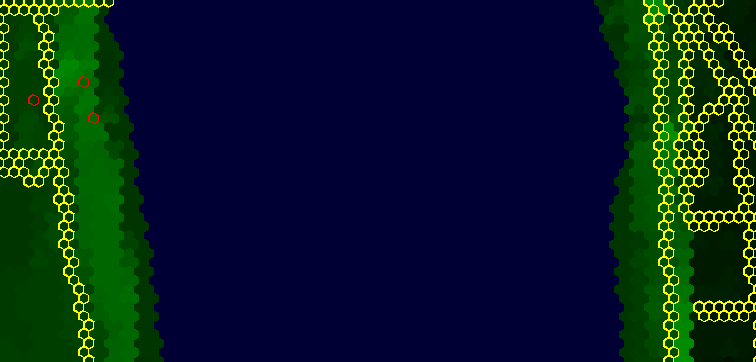
\includegraphics[width=120mm]{figuras/cap5/visor.png}
 \caption{Río Mississippi visto por el visor bidimensional}
\end{figure}

Los colores escogidos son: azul para el agua, verde para el terreno no
inundado, borde amarillo para las calles, borde rojo para los refugios, punto
rojo para las personas. La intensidad del color determina su altura, a más
claro el color, mayor es la altura de la casilla -se ignora la profundidad,
sólo se tiene en cuenta la altura-.

\section*{Estadísticas}
Siguiendo la misma estrategia que los demás objetos que se actualizan
periódicamente, hemos diseñado un agente estadístico que se encarga de recoger
información de cada estado de la simulación.

Recogiendo la información deseada, en nuestro caso, el estado de las personas,
y el tiempo de la simulación, podemos hacer una evaluación estadística de la
evolución de la inundación, sabiendo cuales han sido las zonas donde mas
personas han perecido, o salvado y la hora en la que sucedió.
\subsection*{Múltiples Escenarios}
%Soporte para varios escenarios
Nuestra simulación puede tener mas de un escenario, por ello necesitamos
identificar de que escenario estamos recogiendo los datos, esto lo realizamos
simplemente añadiendo una columna con el identificador del escenario.
\subsection*{Ficheros CVS}
%Es lo mas comodo para las estadisticas
Los ficheros CSV\footnote{Valores Separados por Coma :
\url{http://es.wikipedia.org/wiki/CSV}} son muy fáciles de escribir y leer y la
forma mas simple de almacenar información. Por ello los hace ideales para
nuestro propósito de recoger una serie de estadísticas y guardarlas en un
fichero que sigue una forma estándar de almacenar los datos y que es reconocida
por la mayoría de hojas de cálculo y fácilmente se pueden generar gráficas a 
partir de estos ficheros.
%%% Local Variables:
%%% mode: latex
%%% TeX-master: "../dissim"
%%% End: % Metodología e implementación
% Resultados

\chapter*{Resultados} \label{cap6}
\addcontentsline{toc}{chapter}{Resultados}

\begin{flushright}
\begin{minipage}{7.85cm}
    {\em Si buscas resultados distintos, no hagas siempre lo mismo.} \\ Albert
    Einstein
\end{minipage}
\end{flushright}

\vspace*{5mm}

\section*{Escalabilidad}
%Lo podemos echar a correr en varias maquinas, eso es cosa de jade
\section*{Resultados}
%echamos a correr el simulador y comentamos la jugada
\subsection*{Visualización de Resultados}
%Ventanitas del simulador o capturas de google earth
\section*{Simulación frente Realidad}
%Es cuestion de preparar un escenario de nueva orleans y comparar con la
%bibliografia

%%% Local Variables:
%%% mode: latex
%%% TeX-master: "../dissim"
%%% End: % Resultados
% Conclusiones y trabajo futuro

\chapter*{Conclusiones} \label{cap7}
\addcontentsline{toc}{chapter}{Conclusiones}

\begin{flushright}
\begin{minipage}{7.85cm}
    {\em Blah blah blah.} \\  Alguien
\end{minipage}
\end{flushright}

\vspace*{5mm}

\section*{Conclusiones}

Lorem ipsum dolor sit amet, consectetur adipiscing elit. Vestibulum placerat
urna egestas magna blandit quis tristique libero tincidunt. Aliquam erat
volutpat. Mauris nec purus eu justo ultrices tempus quis nec justo. In hac
habitasse platea dictumst. Vestibulum risus nisl, bibendum id pellentesque et,
interdum in dui. Etiam mattis, odio volutpat facilisis imperdiet, neque lectus
tempor nulla, vel pharetra elit tortor eu turpis. Pellentesque habitant morbi
tristique senectus et netus et malesuada fames ac turpis egestas. Nunc arcu
ligula, pretium nec bibendum at, porta nec justo. Duis ultrices tristique odio,
sit amet elementum nisl mattis eu. Maecenas convallis purus a diam dictum vitae
consectetur lacus tempor. Aenean sed orci mauris, id scelerisque arcu. Nulla
tristique sollicitudin tortor vel pulvinar. Cras egestas aliquet nisi
condimentum placerat. Cras pulvinar dolor eget eros iaculis commodo fermentum
ipsum consectetur. Phasellus quis neque quis tellus faucibus feugiat. Proin
rhoncus lectus lectus, eu rutrum nunc. Quisque sed ipsum vitae ligula gravida
viverra. In ut libero est, a venenatis diam.

Pellentesque nec nulla ut lacus blandit venenatis. Morbi vitae enim dolor.
Vestibulum euismod odio non justo lobortis et lobortis magna mollis. Cras
aliquet dapibus enim, nec interdum mi interdum sed. Sed porttitor magna ut dolor
interdum pellentesque. Aliquam erat volutpat. Vestibulum ante ipsum primis in
faucibus orci luctus et ultrices posuere cubilia Curae; Cras id felis neque.
Suspendisse sem urna, euismod nec pharetra et, egestas quis nunc. Maecenas
blandit viverra nisl eu dapibus. Ut auctor nunc et dui tincidunt volutpat. In ut
metus nibh. Lorem ipsum dolor sit amet, consectetur adipiscing elit. Cras at
quam non lectus laoreet sollicitudin vel eget ligula. Lorem ipsum dolor sit
amet, consectetur adipiscing elit. Curabitur sed diam dolor, id vestibulum arcu.
Cum sociis natoque penatibus et magnis dis parturient montes, nascetur ridiculus
mus. Integer id vulputate leo. Phasellus feugiat, purus sit amet lacinia
consequat, urna risus feugiat lacus, in lobortis velit mi et orci. Vivamus est
est, dapibus sed rhoncus et, facilisis vitae sapien.

Mauris tempor bibendum odio, at varius erat tristique vitae. Duis sit amet erat
non nisi convallis condimentum ut ut nulla. Fusce eros orci, egestas a congue
at, egestas ut ligula. Praesent dolor dolor, mollis vitae tincidunt in, lobortis
vitae odio. Nullam id nisl ipsum. Cras vel arcu mattis lectus ornare ornare eu a
ligula. Cras non enim et risus aliquam aliquam sit amet a magna. Curabitur id
gravida lectus. Curabitur semper arcu in dolor laoreet sed molestie sapien
fringilla. Duis et lectus nisi, sit amet auctor dui. Nullam accumsan diam in
purus scelerisque in commodo turpis sollicitudin. Donec congue egestas lectus a
semper. Aliquam ullamcorper nibh eget massa fermentum hendrerit. Morbi felis
risus, cursus semper sollicitudin ut, consequat quis orci. Duis ante lacus,
varius ac consequat feugiat, gravida ac enim. Curabitur accumsan aliquet
placerat. Phasellus ut mauris nisi. In hac habitasse platea dictumst. Mauris
vehicula fringilla dolor, ut sodales mauris congue a. In hac habitasse platea
dictumst.

Vestibulum quam diam, rhoncus rhoncus tristique et, volutpat sed ipsum. Proin
varius tristique magna, eu varius turpis malesuada at. Nam dignissim tempor
augue a tristique. Fusce velit tortor, pulvinar quis mollis sed, iaculis ac
urna. Donec urna diam, consectetur sed lacinia quis, consectetur suscipit
mauris. Nullam malesuada faucibus porttitor. Nulla felis justo, lobortis sed
varius id, dictum vel metus. Nam nunc arcu, imperdiet in malesuada ut, mollis
eget neque. Quisque felis lacus, vulputate sit amet fringilla sed, feugiat nec
tortor. Vestibulum ante ipsum primis in faucibus orci luctus et ultrices posuere
cubilia Curae; In hac habitasse platea dictumst. Integer et nisi eros, quis
pulvinar felis. Suspendisse semper tempor porta. Donec justo tellus, iaculis
eget lacinia et, vulputate tincidunt urna. Lorem ipsum dolor sit amet,
consectetur adipiscing elit. Sed sem tellus, sodales id tincidunt at, gravida ut
eros.

Nam turpis erat, pulvinar et porttitor euismod, ullamcorper sit amet ante.
Suspendisse dapibus dapibus tellus, vel iaculis tortor congue adipiscing.
Vestibulum ante ipsum primis in faucibus orci luctus et ultrices posuere cubilia
Curae; Sed nec diam vel nisl aliquam blandit. Proin massa quam, rutrum nec
imperdiet molestie, hendrerit non est. Cras in dapibus lorem. Suspendisse eget
tortor at risus hendrerit ultrices sed ut magna. Pellentesque libero dolor,
eleifend vitae scelerisque sit amet, lobortis egestas justo. Integer nisl dui,
ornare a scelerisque eget, faucibus vel risus. Pellentesque habitant morbi
tristique senectus et netus et malesuada fames ac turpis egestas. Maecenas
sodales, mauris in condimentum faucibus, lectus lectus laoreet felis, id gravida
ipsum orci eu quam. Nunc tincidunt, ante a blandit lacinia, felis eros
consectetur est, sed rutrum libero eros eget libero.

%%% Local Variables:
%%% mode: latex
%%% TeX-master: "../dea"
%%% End: % Conclusiones y trabajo futuro

%%  Apéndices
%%%%%%%%%%%%%%%%%%%%%%%%%%%%%%%%%%%%%%%%%%%%%%%%%%%%%%%%%%%%%%%%%%%%%%
\appendix
% Licencia del proyecto

\chapter*{Licencia del Simulador} \label{ap1}
\addcontentsline{toc}{chapter}{Licencia}

\vspace*{5mm}

\begin{center}
{\parindent 0in

{\Large \sc \textbf{GNU GENERAL PUBLIC LICENSE}}

Version 3, 29 June 2007

Copyright \copyright\  2007 Free Software Foundation, Inc.
\texttt{http://fsf.org/}

\bigskip
Everyone is permitted to copy and distribute verbatim copies of this

license document, but changing it is not allowed.}

\end{center}

\begin{center}
{\Large \sc Terms and Conditions}
\end{center}


\begin{enumerate}

\addtocounter{enumi}{-1}

\item Definitions.

``This License'' refers to version 3 of the GNU General Public License.

``Copyright'' also means copyright-like laws that apply to other kinds of
works, such as semiconductor masks.

``The Program'' refers to any copyrightable work licensed under this
License.  Each licensee is addressed as ``you''.  ``Licensees'' and
``recipients'' may be individuals or organizations.

To ``modify'' a work means to copy from or adapt all or part of the work
in a fashion requiring copyright permission, other than the making of an
exact copy.  The resulting work is called a ``modified version'' of the
earlier work or a work ``based on'' the earlier work.

A ``covered work'' means either the unmodified Program or a work based
on the Program.

To ``propagate'' a work means to do anything with it that, without
permission, would make you directly or secondarily liable for
infringement under applicable copyright law, except executing it on a
computer or modifying a private copy.  Propagation includes copying,
distribution (with or without modification), making available to the
public, and in some countries other activities as well.

To ``convey'' a work means any kind of propagation that enables other
parties to make or receive copies.  Mere interaction with a user through
a computer network, with no transfer of a copy, is not conveying.

An interactive user interface displays ``Appropriate Legal Notices''
to the extent that it includes a convenient and prominently visible
feature that (1) displays an appropriate copyright notice, and (2)
tells the user that there is no warranty for the work (except to the
extent that warranties are provided), that licensees may convey the
work under this License, and how to view a copy of this License.  If
the interface presents a list of user commands or options, such as a
menu, a prominent item in the list meets this criterion.

\item Source Code.

The ``source code'' for a work means the preferred form of the work
for making modifications to it.  ``Object code'' means any non-source
form of a work.

A ``Standard Interface'' means an interface that either is an official
standard defined by a recognized standards body, or, in the case of
interfaces specified for a particular programming language, one that
is widely used among developers working in that language.

The ``System Libraries'' of an executable work include anything, other
than the work as a whole, that (a) is included in the normal form of
packaging a Major Component, but which is not part of that Major
Component, and (b) serves only to enable use of the work with that
Major Component, or to implement a Standard Interface for which an
implementation is available to the public in source code form.  A
``Major Component'', in this context, means a major essential component
(kernel, window system, and so on) of the specific operating system
(if any) on which the executable work runs, or a compiler used to
produce the work, or an object code interpreter used to run it.

The ``Corresponding Source'' for a work in object code form means all
the source code needed to generate, install, and (for an executable
work) run the object code and to modify the work, including scripts to
control those activities.  However, it does not include the work's
System Libraries, or general-purpose tools or generally available free
programs which are used unmodified in performing those activities but
which are not part of the work.  For example, Corresponding Source
includes interface definition files associated with source files for
the work, and the source code for shared libraries and dynamically
linked subprograms that the work is specifically designed to require,
such as by intimate data communication or control flow between those
subprograms and other parts of the work.

The Corresponding Source need not include anything that users
can regenerate automatically from other parts of the Corresponding
Source.

The Corresponding Source for a work in source code form is that
same work.

\item Basic Permissions.

All rights granted under this License are granted for the term of
copyright on the Program, and are irrevocable provided the stated
conditions are met.  This License explicitly affirms your unlimited
permission to run the unmodified Program.  The output from running a
covered work is covered by this License only if the output, given its
content, constitutes a covered work.  This License acknowledges your
rights of fair use or other equivalent, as provided by copyright law.

You may make, run and propagate covered works that you do not
convey, without conditions so long as your license otherwise remains
in force.  You may convey covered works to others for the sole purpose
of having them make modifications exclusively for you, or provide you
with facilities for running those works, provided that you comply with
the terms of this License in conveying all material for which you do
not control copyright.  Those thus making or running the covered works
for you must do so exclusively on your behalf, under your direction
and control, on terms that prohibit them from making any copies of
your copyrighted material outside their relationship with you.

Conveying under any other circumstances is permitted solely under
the conditions stated below.  Sublicensing is not allowed; section 10
makes it unnecessary.

\item Protecting Users' Legal Rights From Anti-Circumvention Law.

No covered work shall be deemed part of an effective technological
measure under any applicable law fulfilling obligations under article
11 of the WIPO copyright treaty adopted on 20 December 1996, or
similar laws prohibiting or restricting circumvention of such
measures.

When you convey a covered work, you waive any legal power to forbid
circumvention of technological measures to the extent such circumvention
is effected by exercising rights under this License with respect to
the covered work, and you disclaim any intention to limit operation or
modification of the work as a means of enforcing, against the work's
users, your or third parties' legal rights to forbid circumvention of
technological measures.

\item Conveying Verbatim Copies.

You may convey verbatim copies of the Program's source code as you
receive it, in any medium, provided that you conspicuously and
appropriately publish on each copy an appropriate copyright notice;
keep intact all notices stating that this License and any
non-permissive terms added in accord with section 7 apply to the code;
keep intact all notices of the absence of any warranty; and give all
recipients a copy of this License along with the Program.

You may charge any price or no price for each copy that you convey,
and you may offer support or warranty protection for a fee.

\item Conveying Modified Source Versions.

You may convey a work based on the Program, or the modifications to
produce it from the Program, in the form of source code under the
terms of section 4, provided that you also meet all of these conditions:
  \begin{enumerate}
  \item The work must carry prominent notices stating that you modified
  it, and giving a relevant date.

  \item The work must carry prominent notices stating that it is
  released under this License and any conditions added under section
  7.  This requirement modifies the requirement in section 4 to
  ``keep intact all notices''.

  \item You must license the entire work, as a whole, under this
  License to anyone who comes into possession of a copy.  This
  License will therefore apply, along with any applicable section 7
  additional terms, to the whole of the work, and all its parts,
  regardless of how they are packaged.  This License gives no
  permission to license the work in any other way, but it does not
  invalidate such permission if you have separately received it.

  \item If the work has interactive user interfaces, each must display
  Appropriate Legal Notices; however, if the Program has interactive
  interfaces that do not display Appropriate Legal Notices, your
  work need not make them do so.
\end{enumerate}
A compilation of a covered work with other separate and independent
works, which are not by their nature extensions of the covered work,
and which are not combined with it such as to form a larger program,
in or on a volume of a storage or distribution medium, is called an
``aggregate'' if the compilation and its resulting copyright are not
used to limit the access or legal rights of the compilation's users
beyond what the individual works permit.  Inclusion of a covered work
in an aggregate does not cause this License to apply to the other
parts of the aggregate.

\item Conveying Non-Source Forms.

You may convey a covered work in object code form under the terms
of sections 4 and 5, provided that you also convey the
machine-readable Corresponding Source under the terms of this License,
in one of these ways:
  \begin{enumerate}
  \item Convey the object code in, or embodied in, a physical product
  (including a physical distribution medium), accompanied by the
  Corresponding Source fixed on a durable physical medium
  customarily used for software interchange.

  \item Convey the object code in, or embodied in, a physical product
  (including a physical distribution medium), accompanied by a
  written offer, valid for at least three years and valid for as
  long as you offer spare parts or customer support for that product
  model, to give anyone who possesses the object code either (1) a
  copy of the Corresponding Source for all the software in the
  product that is covered by this License, on a durable physical
  medium customarily used for software interchange, for a price no
  more than your reasonable cost of physically performing this
  conveying of source, or (2) access to copy the
  Corresponding Source from a network server at no charge.

  \item Convey individual copies of the object code with a copy of the
  written offer to provide the Corresponding Source.  This
  alternative is allowed only occasionally and noncommercially, and
  only if you received the object code with such an offer, in accord
  with subsection 6b.

  \item Convey the object code by offering access from a designated
  place (gratis or for a charge), and offer equivalent access to the
  Corresponding Source in the same way through the same place at no
  further charge.  You need not require recipients to copy the
  Corresponding Source along with the object code.  If the place to
  copy the object code is a network server, the Corresponding Source
  may be on a different server (operated by you or a third party)
  that supports equivalent copying facilities, provided you maintain
  clear directions next to the object code saying where to find the
  Corresponding Source.  Regardless of what server hosts the
  Corresponding Source, you remain obligated to ensure that it is
  available for as long as needed to satisfy these requirements.

  \item Convey the object code using peer-to-peer transmission, provided
  you inform other peers where the object code and Corresponding
  Source of the work are being offered to the general public at no
  charge under subsection 6d.
  \end{enumerate}

A separable portion of the object code, whose source code is excluded
from the Corresponding Source as a System Library, need not be
included in conveying the object code work.

A ``User Product'' is either (1) a ``consumer product'', which means any
tangible personal property which is normally used for personal, family,
or household purposes, or (2) anything designed or sold for incorporation
into a dwelling.  In determining whether a product is a consumer product,
doubtful cases shall be resolved in favor of coverage.  For a particular
product received by a particular user, ``normally used'' refers to a
typical or common use of that class of product, regardless of the status
of the particular user or of the way in which the particular user
actually uses, or expects or is expected to use, the product.  A product
is a consumer product regardless of whether the product has substantial
commercial, industrial or non-consumer uses, unless such uses represent
the only significant mode of use of the product.

``Installation Information'' for a User Product means any methods,
procedures, authorization keys, or other information required to install
and execute modified versions of a covered work in that User Product from
a modified version of its Corresponding Source.  The information must
suffice to ensure that the continued functioning of the modified object
code is in no case prevented or interfered with solely because
modification has been made.

If you convey an object code work under this section in, or with, or
specifically for use in, a User Product, and the conveying occurs as
part of a transaction in which the right of possession and use of the
User Product is transferred to the recipient in perpetuity or for a
fixed term (regardless of how the transaction is characterized), the
Corresponding Source conveyed under this section must be accompanied
by the Installation Information.  But this requirement does not apply
if neither you nor any third party retains the ability to install
modified object code on the User Product (for example, the work has
been installed in ROM).

The requirement to provide Installation Information does not include a
requirement to continue to provide support service, warranty, or updates
for a work that has been modified or installed by the recipient, or for
the User Product in which it has been modified or installed.  Access to a
network may be denied when the modification itself materially and
adversely affects the operation of the network or violates the rules and
protocols for communication across the network.

Corresponding Source conveyed, and Installation Information provided,
in accord with this section must be in a format that is publicly
documented (and with an implementation available to the public in
source code form), and must require no special password or key for
unpacking, reading or copying.

\item Additional Terms.

``Additional permissions'' are terms that supplement the terms of this
License by making exceptions from one or more of its conditions.
Additional permissions that are applicable to the entire Program shall
be treated as though they were included in this License, to the extent
that they are valid under applicable law.  If additional permissions
apply only to part of the Program, that part may be used separately
under those permissions, but the entire Program remains governed by
this License without regard to the additional permissions.

When you convey a copy of a covered work, you may at your option
remove any additional permissions from that copy, or from any part of
it.  (Additional permissions may be written to require their own
removal in certain cases when you modify the work.)  You may place
additional permissions on material, added by you to a covered work,
for which you have or can give appropriate copyright permission.

Notwithstanding any other provision of this License, for material you
add to a covered work, you may (if authorized by the copyright holders of
that material) supplement the terms of this License with terms:
  \begin{enumerate}
  \item Disclaiming warranty or limiting liability differently from the
  terms of sections 15 and 16 of this License; or

  \item Requiring preservation of specified reasonable legal notices or
  author attributions in that material or in the Appropriate Legal
  Notices displayed by works containing it; or

  \item Prohibiting misrepresentation of the origin of that material, or
  requiring that modified versions of such material be marked in
  reasonable ways as different from the original version; or

  \item Limiting the use for publicity purposes of names of licensors or
  authors of the material; or

  \item Declining to grant rights under trademark law for use of some
  trade names, trademarks, or service marks; or

  \item Requiring indemnification of licensors and authors of that
  material by anyone who conveys the material (or modified versions of
  it) with contractual assumptions of liability to the recipient, for
  any liability that these contractual assumptions directly impose on
  those licensors and authors.
  \end{enumerate}

All other non-permissive additional terms are considered ``further
restrictions'' within the meaning of section 10.  If the Program as you
received it, or any part of it, contains a notice stating that it is
governed by this License along with a term that is a further
restriction, you may remove that term.  If a license document contains
a further restriction but permits relicensing or conveying under this
License, you may add to a covered work material governed by the terms
of that license document, provided that the further restriction does
not survive such relicensing or conveying.

If you add terms to a covered work in accord with this section, you
must place, in the relevant source files, a statement of the
additional terms that apply to those files, or a notice indicating
where to find the applicable terms.

Additional terms, permissive or non-permissive, may be stated in the
form of a separately written license, or stated as exceptions;
the above requirements apply either way.

\item Termination.

You may not propagate or modify a covered work except as expressly
provided under this License.  Any attempt otherwise to propagate or
modify it is void, and will automatically terminate your rights under
this License (including any patent licenses granted under the third
paragraph of section 11).

However, if you cease all violation of this License, then your
license from a particular copyright holder is reinstated (a)
provisionally, unless and until the copyright holder explicitly and
finally terminates your license, and (b) permanently, if the copyright
holder fails to notify you of the violation by some reasonable means
prior to 60 days after the cessation.

Moreover, your license from a particular copyright holder is
reinstated permanently if the copyright holder notifies you of the
violation by some reasonable means, this is the first time you have
received notice of violation of this License (for any work) from that
copyright holder, and you cure the violation prior to 30 days after
your receipt of the notice.

Termination of your rights under this section does not terminate the
licenses of parties who have received copies or rights from you under
this License.  If your rights have been terminated and not permanently
reinstated, you do not qualify to receive new licenses for the same
material under section 10.

\item Acceptance Not Required for Having Copies.

You are not required to accept this License in order to receive or
run a copy of the Program.  Ancillary propagation of a covered work
occurring solely as a consequence of using peer-to-peer transmission
to receive a copy likewise does not require acceptance.  However,
nothing other than this License grants you permission to propagate or
modify any covered work.  These actions infringe copyright if you do
not accept this License.  Therefore, by modifying or propagating a
covered work, you indicate your acceptance of this License to do so.

\item Automatic Licensing of Downstream Recipients.

Each time you convey a covered work, the recipient automatically
receives a license from the original licensors, to run, modify and
propagate that work, subject to this License.  You are not responsible
for enforcing compliance by third parties with this License.

An ``entity transaction'' is a transaction transferring control of an
organization, or substantially all assets of one, or subdividing an
organization, or merging organizations.  If propagation of a covered
work results from an entity transaction, each party to that
transaction who receives a copy of the work also receives whatever
licenses to the work the party's predecessor in interest had or could
give under the previous paragraph, plus a right to possession of the
Corresponding Source of the work from the predecessor in interest, if
the predecessor has it or can get it with reasonable efforts.

You may not impose any further restrictions on the exercise of the
rights granted or affirmed under this License.  For example, you may
not impose a license fee, royalty, or other charge for exercise of
rights granted under this License, and you may not initiate litigation
(including a cross-claim or counterclaim in a lawsuit) alleging that
any patent claim is infringed by making, using, selling, offering for
sale, or importing the Program or any portion of it.

\item Patents.

A ``contributor'' is a copyright holder who authorizes use under this
License of the Program or a work on which the Program is based.  The
work thus licensed is called the contributor's ``contributor version''.

A contributor's ``essential patent claims'' are all patent claims
owned or controlled by the contributor, whether already acquired or
hereafter acquired, that would be infringed by some manner, permitted
by this License, of making, using, or selling its contributor version,
but do not include claims that would be infringed only as a
consequence of further modification of the contributor version.  For
purposes of this definition, ``control'' includes the right to grant
patent sublicenses in a manner consistent with the requirements of
this License.

Each contributor grants you a non-exclusive, worldwide, royalty-free
patent license under the contributor's essential patent claims, to
make, use, sell, offer for sale, import and otherwise run, modify and
propagate the contents of its contributor version.

In the following three paragraphs, a ``patent license'' is any express
agreement or commitment, however denominated, not to enforce a patent
(such as an express permission to practice a patent or covenant not to
sue for patent infringement).  To ``grant'' such a patent license to a
party means to make such an agreement or commitment not to enforce a
patent against the party.

If you convey a covered work, knowingly relying on a patent license,
and the Corresponding Source of the work is not available for anyone
to copy, free of charge and under the terms of this License, through a
publicly available network server or other readily accessible means,
then you must either (1) cause the Corresponding Source to be so
available, or (2) arrange to deprive yourself of the benefit of the
patent license for this particular work, or (3) arrange, in a manner
consistent with the requirements of this License, to extend the patent
license to downstream recipients.  ``Knowingly relying'' means you have
actual knowledge that, but for the patent license, your conveying the
covered work in a country, or your recipient's use of the covered work
in a country, would infringe one or more identifiable patents in that
country that you have reason to believe are valid.

If, pursuant to or in connection with a single transaction or
arrangement, you convey, or propagate by procuring conveyance of, a
covered work, and grant a patent license to some of the parties
receiving the covered work authorizing them to use, propagate, modify
or convey a specific copy of the covered work, then the patent license
you grant is automatically extended to all recipients of the covered
work and works based on it.

A patent license is ``discriminatory'' if it does not include within
the scope of its coverage, prohibits the exercise of, or is
conditioned on the non-exercise of one or more of the rights that are
specifically granted under this License.  You may not convey a covered
work if you are a party to an arrangement with a third party that is
in the business of distributing software, under which you make payment
to the third party based on the extent of your activity of conveying
the work, and under which the third party grants, to any of the
parties who would receive the covered work from you, a discriminatory
patent license (a) in connection with copies of the covered work
conveyed by you (or copies made from those copies), or (b) primarily
for and in connection with specific products or compilations that
contain the covered work, unless you entered into that arrangement,
or that patent license was granted, prior to 28 March 2007.

Nothing in this License shall be construed as excluding or limiting
any implied license or other defenses to infringement that may
otherwise be available to you under applicable patent law.

\item No Surrender of Others' Freedom.

If conditions are imposed on you (whether by court order, agreement or
otherwise) that contradict the conditions of this License, they do not
excuse you from the conditions of this License.  If you cannot convey a
covered work so as to satisfy simultaneously your obligations under this
License and any other pertinent obligations, then as a consequence you may
not convey it at all.  For example, if you agree to terms that obligate you
to collect a royalty for further conveying from those to whom you convey
the Program, the only way you could satisfy both those terms and this
License would be to refrain entirely from conveying the Program.

\item Use with the GNU Affero General Public License.

Notwithstanding any other provision of this License, you have
permission to link or combine any covered work with a work licensed
under version 3 of the GNU Affero General Public License into a single
combined work, and to convey the resulting work.  The terms of this
License will continue to apply to the part which is the covered work,
but the special requirements of the GNU Affero General Public License,
section 13, concerning interaction through a network will apply to the
combination as such.

\item Revised Versions of this License.

The Free Software Foundation may publish revised and/or new versions of
the GNU General Public License from time to time.  Such new versions will
be similar in spirit to the present version, but may differ in detail to
address new problems or concerns.

Each version is given a distinguishing version number.  If the
Program specifies that a certain numbered version of the GNU General
Public License ``or any later version'' applies to it, you have the
option of following the terms and conditions either of that numbered
version or of any later version published by the Free Software
Foundation.  If the Program does not specify a version number of the
GNU General Public License, you may choose any version ever published
by the Free Software Foundation.

If the Program specifies that a proxy can decide which future
versions of the GNU General Public License can be used, that proxy's
public statement of acceptance of a version permanently authorizes you
to choose that version for the Program.

Later license versions may give you additional or different
permissions.  However, no additional obligations are imposed on any
author or copyright holder as a result of your choosing to follow a
later version.

\item Disclaimer of Warranty.

\begin{sloppypar}
 THERE IS NO WARRANTY FOR THE PROGRAM, TO THE EXTENT PERMITTED BY
 APPLICABLE LAW.  EXCEPT WHEN OTHERWISE STATED IN WRITING THE
 COPYRIGHT HOLDERS AND/OR OTHER PARTIES PROVIDE THE PROGRAM ``AS IS''
 WITHOUT WARRANTY OF ANY KIND, EITHER EXPRESSED OR IMPLIED,
 INCLUDING, BUT NOT LIMITED TO, THE IMPLIED WARRANTIES OF
 MERCHANTABILITY AND FITNESS FOR A PARTICULAR PURPOSE.  THE ENTIRE
 RISK AS TO THE QUALITY AND PERFORMANCE OF THE PROGRAM IS WITH YOU.
 SHOULD THE PROGRAM PROVE DEFECTIVE, YOU ASSUME THE COST OF ALL
 NECESSARY SERVICING, REPAIR OR CORRECTION.
\end{sloppypar}

\item Limitation of Liability.

 IN NO EVENT UNLESS REQUIRED BY APPLICABLE LAW OR AGREED TO IN
 WRITING WILL ANY COPYRIGHT HOLDER, OR ANY OTHER PARTY WHO MODIFIES
 AND/OR CONVEYS THE PROGRAM AS PERMITTED ABOVE, BE LIABLE TO YOU FOR
 DAMAGES, INCLUDING ANY GENERAL, SPECIAL, INCIDENTAL OR CONSEQUENTIAL
 DAMAGES ARISING OUT OF THE USE OR INABILITY TO USE THE PROGRAM
 (INCLUDING BUT NOT LIMITED TO LOSS OF DATA OR DATA BEING RENDERED
 INACCURATE OR LOSSES SUSTAINED BY YOU OR THIRD PARTIES OR A FAILURE
 OF THE PROGRAM TO OPERATE WITH ANY OTHER PROGRAMS), EVEN IF SUCH
 HOLDER OR OTHER PARTY HAS BEEN ADVISED OF THE POSSIBILITY OF SUCH
 DAMAGES.

\item Interpretation of Sections 15 and 16.

If the disclaimer of warranty and limitation of liability provided
above cannot be given local legal effect according to their terms,
reviewing courts shall apply local law that most closely approximates
an absolute waiver of all civil liability in connection with the
Program, unless a warranty or assumption of liability accompanies a
copy of the Program in return for a fee.

\begin{center}
{\Large\sc End of Terms and Conditions}

\bigskip
How to Apply These Terms to Your New Programs
\end{center}

If you develop a new program, and you want it to be of the greatest
possible use to the public, the best way to achieve this is to make it
free software which everyone can redistribute and change under these terms.

To do so, attach the following notices to the program.  It is safest
to attach them to the start of each source file to most effectively
state the exclusion of warranty; and each file should have at least
the ``copyright'' line and a pointer to where the full notice is found.

{\footnotesize
\begin{verbatim}
<one line to give the program's name and a brief idea of what it does.>

Copyright (C) <textyear>  <name of author>

This program is free software: you can redistribute it and/or modify
it under the terms of the GNU General Public License as published by
the Free Software Foundation, either version 3 of the License, or
(at your option) any later version.

This program is distributed in the hope that it will be useful,
but WITHOUT ANY WARRANTY; without even the implied warranty of
MERCHANTABILITY or FITNESS FOR A PARTICULAR PURPOSE.  See the
GNU General Public License for more details.

You should have received a copy of the GNU General Public License
along with this program.  If not, see <http://www.gnu.org/licenses/>.
\end{verbatim}
}

Also add information on how to contact you by electronic and paper mail.

If the program does terminal interaction, make it output a short
notice like this when it starts in an interactive mode:

{\footnotesize
\begin{verbatim}
<program>  Copyright (C) <year>  <name of author>

This program comes with ABSOLUTELY NO WARRANTY; for details type `show w'.
This is free software, and you are welcome to redistribute it
under certain conditions; type `show c' for details.
\end{verbatim}
}

The hypothetical commands {\tt show w} and {\tt show c} should show
the appropriate
parts of the General Public License.  Of course, your program's commands
might be different; for a GUI interface, you would use an ``about box''.

You should also get your employer (if you work as a programmer) or
school, if any, to sign a ``copyright disclaimer'' for the program, if
necessary.  For more information on this, and how to apply and follow
the GNU GPL, see \texttt{http://www.gnu.org/licenses/}.

The GNU General Public License does not permit incorporating your
program into proprietary programs.  If your program is a subroutine
library, you may consider it more useful to permit linking proprietary
applications with the library.  If this is what you want to do, use
the GNU Lesser General Public License instead of this License.  But
first, please read \texttt{http://www.gnu.org/philosophy/why-not-lgpl.html}.

\end{enumerate}

% \end{document}
  % Licencia
\chapter{Concurso Universitario de Software Libre} \label{ap2}
%\addcontentsline{toc}{chapter}{Concurso Universitario de Software Libre}

\vspace*{5mm}

\section{Introducción}

En este apéndice comentamos y exponemos los datos y bases del Concurso
Universitario de Software Libre (CUSL), en concreto en lo referente a su cuarta
edición, que es en la que inscribimos el proyecto.

Toda esta información ha sido extraída de la web del concurso:
\url{http://www.concursosoftwarelibre.org/}

\subsection{¿Qué es...?}

Es un concurso de desarrollo de software, hardware y documentación técnica
libre, en el que pueden participar estudiantes universitarios de primer,
segundo y tercer ciclo; así como estudiantes no universitarios de bachillerato,
grado medio y superior del ámbito estatal español.

Para liberar los proyectos se emplea principalmente la forja de
RedIRIS\footnote{Forja IRIS-Libre: \url{https://forja.rediris.es/}}. Los
participantes además disponen de un blog donde contarán su experiencia en el
desarrollo durante el curso académico.

\subsection{¿Qué Objetivos Persigue?}

El objetivo principal del Concurso Universitario de Software Libre es fomentar
la creación, y contribuir a la consolidación, de la comunidad del Software Libre
en la Universidad.

\subsection{Premios Locales}

Además del Premio General a nivel estatal, desde la segunda edición del
concurso, existen los Premios Locales.

La Universidad e instituciones vinculadas al mundo del software libre están
invitadas a formar parte de la comunidad del Concurso Universitario de Software
Libre.

Para ello disponen de la posibilidad de premiar a los mejores proyectos
participantes de su ámbito, así como de realizar una fase final local mediante
la modalidad de Premio Local.

De esta forma, sus participantes obtendrán un mayor reconocimiento, se dará
máxima visibilidad a las universidades participantes en la comunidad.

\section{Descripción General}

\begin{enumerate}
\item El Concurso Universitario de Software Libre es un concurso de desarrollo
de software, hardware y documentación técnica libre que consiste en la
elaboración y presentación de un proyecto de Software Libre desarrollado
íntegramente con una implementación libre de cualquier lenguaje de programación.
\item El desarrollo del CUSL consta de las siguientes fases:
    \begin{enumerate}
    \item Fase de inscripción.
    \item Fase de desarrollo.
    \item Fase final.
    \end{enumerate}
\item El máximo de participantes será de tres personas por proyecto.
\item Sólo se podrá participar en un proyecto a la vez.
\item Los proyectos debe estar íntegramente desarrollados con la implementación
en Software Libre de cualquier lenguaje de programación y la licencia elegida
deberá estar comprendida dentro del conjunto de licencias consideradas de
Software Libre por el proyecto GNU (lista en castellano no actualizada). Las
librerías utilizadas también deberán estar bajo este conjunto de licencias.
\item La organización pondrá a disposición de los participantes una forja en la
que se alojarán los proyecto participantes en el CUSL. Los participantes también
dispondrán de un blog, en el que quedará reflejado la evolución del proyecto,
las dificultades encontradas y las decisiones tomadas durante la fase de
desarrollo. Tanto la forja como el blog serán empleados para evaluar la
evolución de los proyectos.
\item El comité de evaluación valorará los siguientes aspectos:
    \begin{enumerate}
    \item {\bf Impacto del proyecto} en la comunidad del software libre y la
    sociedad (30\% de la puntuación). Se valorará positivamente que el proyecto
    genere un tejido social (comunidad) con un interés común en hacer que dicho
    proyecto avance. Esto comprende aspectos como la facilidad para realizar
    trabajos relacionados y/o derivados, su impacto en la esfera socio-política
    y las estrategias de difusión del proyecto en la comunidad del software
    libre.
    \item {\bf Calidad del desarrollo y uso de la forja} (30\% de la
    puntuación). Se valorará positivamente una buena planificación, así como la
    realización de un buen diseño e implementación del proyecto. Una buena
    estrategia en el lanzamiento de versiones será igualmente bien considerada.
    Además, un buen uso de las herramientas disponibles en la forja, tales como
    las listas de correo y el sistema de gestión de código (subversion), serán
    igualmente valorados positivamente.
    \item {\bf Documentación del proyecto} (25\% de la puntuación): La
    documentación es un aspecto importante. Se valorará positivamente la
    realización de documentación de usuario final (detallando la instalación y
    configuración) y de desarrollo (ofreciendo la información pertinente para
    facilitar la realización de trabajos derivados y adaptaciones).
    Grado de finalización (15\% de la puntuación): Se valorará positivamente,
    aunque con menor valor que otros puntos anteriormente descritos, el grado de
    finalización y usabilidad del proyecto.
    \end{enumerate}
\end{enumerate}

\section{Participación}

Nuestro proyecto ha participado en la IV edición del Concurso Universitario de
Software Libre, y nos ha sido otorgada una Mención Especial en el III Premio
Local de Sevilla.  % Concurso Universitario de Software Libre
% \include{apendices/ap3}  % Código fuente del proyecto

%%  Bibliografía
%%%%%%%%%%%%%%%%%%%%%%%%%%%%%%%%%%%%%%%%%%%%%%%%%%%%%%%%%%%%%%%%%%%%%%
\newpage
\addcontentsline{toc}{chapter}{Bibliograf\'ia}
\bibliographystyle{alpha}
\bibliography{bibliografia/referencias.bib}

% chapter 7 de \cite{lamport94}
% para citar se pone  \cite{cite key},

\end{document}
